\chapter{Grundlagen}\label{kap:grundlagen}


\section{Nexys-4-DDR}\label{kap:nexys4}
Das Nexys4 DDR-Board ist eine Entwicklungsplattform, basierend auf dem Artix7-\ac{fpga}
von Xilinx. Es bietet die Möglichkeit mit Hilfe des leistungsstarken \ac{fpga}, des großzügigen, externen Speichers und diversen Anschlussmöglichkeiten
für Peripherie, sämtliche Designs, vom einfachen, kombinatorischen Schaltkreis, bishin zu leistungsstarken eingebetteten Prozessoren, zu realisieren.
Des Weiteren ist auf dem Board Peripherie verbaut, wie zum Beispiel Sensoren, die weitere Nutzungsmöglichkeiten bieten.\\
Das Nexys4 DDR besitzt weiterhin folgende Features:~\cite{digilent}\\
\begin{itemize}
  \item 15,850 logische Slices mit jeweils vier \ac{lut}, welche sechs Eingänge besitzen, sowie acht Flip-Flops.
  \item Es bietet 4,860 Kbit Fast \ac{bram}
  \item Sechs Taktmanagementabschnitte mit jeweils einem \ac{pll}
  \item 240 \ac{dsp}-Slices
  \item Interne Taktraten über 450 MHz
  \item On-Chip-Analog-Digital-Wandler (XADC)
  \item 16 Schalter für den Nutzer
  \item \ac{usb}-\ac{uart}-Brücke
  \item 12-Bit \ac{vga}-Ausgang
  \item 3-Achsen Beschleunigungssensor
  \item 128M DDR2-\ac{sdram} Speicher
  \item Pmod für XADC-Signale
  \item 16 LEDs für den Nutzer
  \item Zwei dreifarbige LEDs
  \item PWM-Audioausgang
  \item Temperatursensor
  \item Digilent \ac{usb}-JTAG Port für \ac{fpga} Programmierung und Kommunikation
  \item Zwei 4-stellige 7-Segment-Anzeigen
  \item Micro SD-Kartenanschluss
  \item PDM-Mikrofon
  \item 10/100 Ethernet-PHY
  \item Vier Pmod-Ports
  \item \ac{usb} HID Host für Mäuse, Tastaturen und Memory Sticks
\end{itemize}



\begin{figure}[H]
\centering
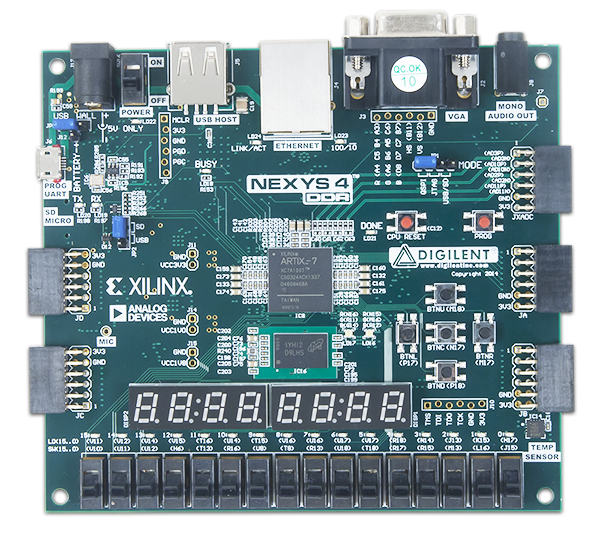
\includegraphics[width=0.6\textwidth]{Hauptteil/nexys-4-ddr-2.png}
\caption{Das Nexys4 DDR-Board von Digilent~\cite{digilent}}\label{fig:nexys4}
\end{figure}



\section{\acl{fpga}}\label{kap:fpga}
Die Xilinx 7-Serie umfasst vier \ac{fpga}-Familien, welche die gesamte Bandbreite an Systemanforderungen abdecken. Diese reicht von kostengünstigen Anwendungen, bis hin zur Hochleistungsanwendung mit High-End-Konnektivitätsbandbreite und Logikkapazität. \\
Die FPGAs der 7-Serie, die auf einer hochmodernen Hochleistungs-HPL-Technologie (HKMG-Technologie) mit 28 nm und High-k-Metal-Gate-Technologie basieren,
 ermöglichen eine beispiellose Steigerung der Systemleistung auf 2,9 Tb/s der Eingabe- und Ausgabe-Bandbreite, 2 Millionen logischer Zellenkapazität und 5,3 TMAC/s DSP,
 wobei 50\% weniger Strom verbraucht wird als bei Geräten der vorherigen Generation, um eine voll programmierbare Alternative zu ASSPs und ASICs zu bieten.\\
 Die Abbildung~\ref{fig:7serie} zeigt den Vergleich der vier \ac{fpga}:~\cite{artix7}\\

 \begin{figure}[H]
 \centering
 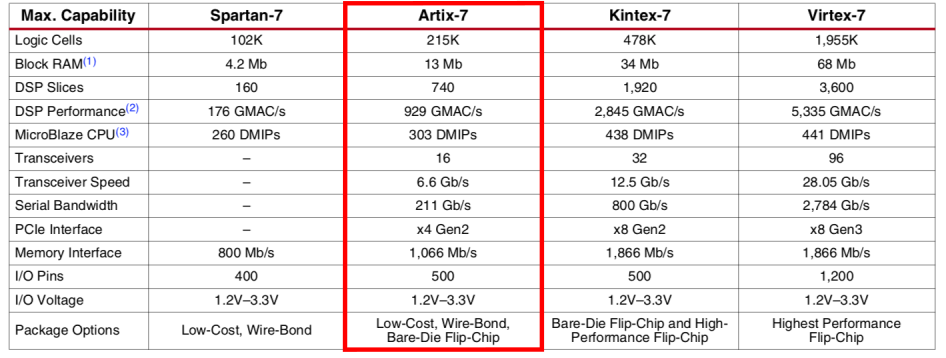
\includegraphics[width=0.8\textwidth]{Hauptteil/7serie.png}
 \caption{Technische Daten des 7-Serie von Xilinx. Der verwendete Artix7 ist rot markiert.~\cite{artix7}}\label{fig:7serie}
 \end{figure}


Bei dem auf dem Board verbauten \ac{fpga} handelt es sich um den  XC7A100T aus der Artix-7-Familie. Diese Baureihe ist optimiert für Low-Power-Anwendungen, welche einen hohen \ac{dsp}- und Logik-Durchsatz erfordern. Einer der großen Vorteile
dieses \ac{fpga} sind die niedrigen Kosten für kostensensitive Anwendungen mit hohem Durchsatz.\\
Die folgende Abbildung zeigt die wichtigsten Daten des verbauten \ac{fpga}:~\cite{artix7}\\


\begin{figure}[H]
\centering
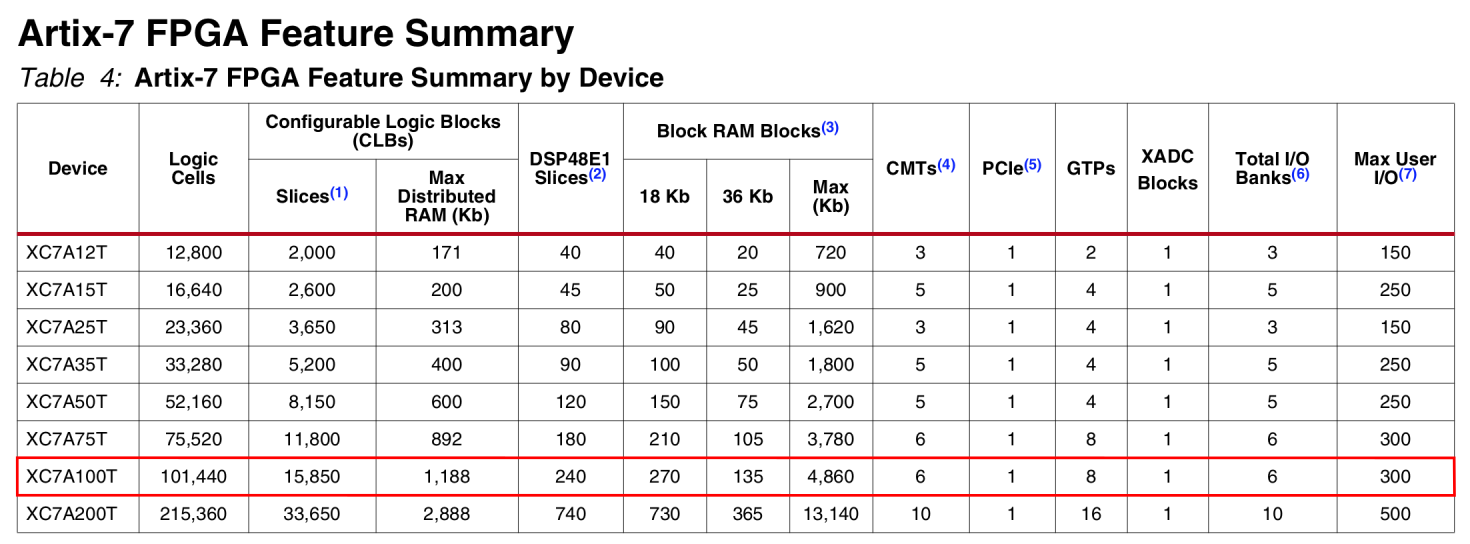
\includegraphics[width=0.8\textwidth]{Hauptteil/artix7.png}
\caption{Technische Daten des Artix7. Der verwendete XC7AC100T ist rot markiert.~\cite{artix7}}\label{fig:artix7}
\end{figure}

\section{Eingebettete Systeme}\label{kap:eingebettetesysteme}

Computer, welche zur Steuerung genutzt werden, nennt man \emph{eingebettete Systeme} (engl. Embedded Systems). In den späten 1960 Jahren wurden diese Systeme erstmalig zur Steuerung in der Kommunikation verwendet. Auf Grund der Tatsache,
dass die Industrie sich in den letzten Jahren unter anderem darauf konzentriert hat, die Systeme immer kleiner zu gestalten, kam es dazu, dass eingebettete Systeme weiterentwickelt wurden. Diese bieten mehr Möglichkeiten für extrem kleine Maschinen.
Durch die steigenden Anforderung an diese Systeme, vor allem im Bezug auf die Netzwerkfähigkeit, wurden diese immer komplexer und benötigen immer mehr Schnittstellen aller Art und einen größeren Speicher als frühere Modelle. Durch diese Anpassungen wurde es
möglich und nötig Betriebssysteme auf diesen Systemen auszuführen, um die steigenden Ressourcen zu verwalten. Bereits in den 70er Jahren wurden die ersten Betriebssysteme für eingebettete Systeme veröffentlich, sodass es heutezutage einige
realisierbare Optionen gibt.\cite{ibm}\\

\textbf{Verschiedene Arten von eingebetteten Systemen}\\

Es gibt eine Menge eingebetteter Systeme, wovon eine Auswahl in der nachfolgenden Aufzählen aufgelistet sind:\cite{ibm}
\begin{itemize}
  \item ETLinux: eine vollständige Linux-Distribution, die auf kleinen industriellen Computern, insbesondere PC / 104-Modulen, ausgeführt werden kann
  \item LEM: eine kleine (<8 MB) Linux-Version für mehrere Benutzer, welche auf 386-Systemen läuft
  \item \ac{loaf}: Eine \emph{Linux on A Floppy}-Distribution, die ebenfalls auf 386-Systemen läuft
  \item uClinux: Linux für Systeme ohne \ac{mmu}. Unterstüutzt die ColdFire-Mikroprozessoren Motorola 68K, MCF5206 und MCF5207
  \item uLinux: kleine Linux-Distribution
  \item ThinLinux: eine minimierte Linux-Distribution für dedizierte Kamera-Server, X-10-Controller, MP3-Player und andere eingebettete Anwendungen
\end{itemize}

\subsection{Vor- und Nachteile von Linux für Embedded Systems}\label{kap:vorundnachteilelinux}

\textbf{Vorteile}\\
Linux-Systeme, welche meistens auf PC-Plattformen laufen, kann es durchaus als verlässliches Arbeitspferd für eingebettete Systeme dienen. Dies geschieht vor allem dadurch, dass Linux die Installation und Verwaltung einfacher macht, indem man sich bei der Entwicklung
auf die Basics beschränkt.\\
So ist das herkömmliche Linux, welches auf einem PC ausgeführt wird, so konfiguriert, dass es mit mit einer Festplatte und viel Arbeitsspeicher umgehen kann, beides besitzt und benötigt eingebettetes System nicht.
 Ein voll ausgestatter Linux-Kernel bentötigt ca. 1 MB Arbeitsspeicher, wovon nur ca 100 KB vom Linux-Mikrokernel verbraucht werden, einschließlich virtuellem Speicher. Betrachetet man dazu noch Dienstprogramme und Netzwerkfunktionen, liegt der benötigte
 Arbeitsspeicher bei ca. 500 KB, welcher unter gewissen Umständen noch reduziert werden kann. Das führt dazu, dass es alles in allem ein leichtgewichtiges Betriebsystem darstellt, welches ideal für eingebettete Systeme ist.\\
 Ein weiterer Vorteil ist es, dass Linux weitestgehend Open-Source ist und dadurch weitaus mehr Treiber und Protokolle zur Verfügung stehen, als bei kommerziellen Systemen. \\
 Das Linux-Betriebssytem besitzt eine einfache Mikrokern-Architektur, bei dem Netzwerk-und Dateisysteme modular auf dem Mikrokern angeordnet sind. Weitere Optionen, wie zum Beispiel Treiber, können kompiliert und dann dem System zur Verfügung gestellt werden
 oder parallel zur Laufzeit als ladbare Module dem Kernel hinzugefügt werden. Daraus folgt, dass ein hochmodulares System entsteht, welches auf ein eingebettetes System angepasst ist.\\
 Um die Ressourcen bestmöglich zu nutzen, erfordert ein Embedded-System, dass auf herkömmliche Programme und Treiber aufgebaut ist, mit denen zum Beispiel gängige Peripheriegeräte und Anwendungen genutzt werden können.\\
 Linux unterstützt Multi-Core-Systeme, welche es besonders für Nutzer interessant macht, welche Anwendungen parallel ausführen wollen und so die Verarbeitungsleistung erhöht wird. Als Beispiel dafür dient die parallele Ausführung eines Linux-System auf einem Prozessor,
  während auf dem anderen Prozessor eine \ac{gui} ausgeführt wird.\cite{ibm}\\

\textbf{Nachteile}\\
Ein wichiger Nachteil beim Ausführen von Linux auf einem eingebetteten System ist es, dass die Linux-Architektur eine Möglichkeit bietet, dass Softwaremodul in
Echtzeit in den Kernel-Space hinzugefügt werden können, welcher für das Zeitmanagement, Hardware-Interrupts und
für das Ausführen von Programmen zuständig ist. Kommt es in dem Kernel-Space zu einem Fehler innerhalb des Codes, kann dieser zu einem Absturz des gesamten
Betriebssystem führen und stellt somit eine ernste Sicherheitslücke für Echtzeitanwendungen dar.\\
Um diese Sicherheitslücke zu schließen, gibt es Standart-\ac{rtos}, welche grundsätzlich für einen Echtzeit-Einsatz konfiguriert sind und eine höhere Zuverlässigkeit bietet. Prozesse erhalten bei Bedarf eine höhere Priorität,
 wenn sie vom Benutzer auf Systemebene gestartet werden. Prozesse erhalten eine ID, damit das Betriebssystem die ausgeführten Programme verfolgen kann. Durch dieses Verfahren erhöht sich die Zuverlässigkeit.\cite{ibm}\\



\subsection{Software-und Hardware-Voraussetzungen}\label{kap:voraussetzungen}

Verschiedene Tools und Programme erweitern die Möglichkeiten des Linux-Kernels, jedoch gibt es eine Minimalanforderung, die ein Embedded-Linux-System benötigt.\\
Dazu zählen:\\
\begin{itemize}
  \item Ein Dienstpogramm, welches das Booten ermöglicht
  \item Den Linux-Mikrokernel, bestehend aus den Dienstprogrammen für Speichermanagement, Prozessmanagement und Timing
  \item Ein Initialisierungsprozess
\end{itemize}

Um letztendlich sinnvolle Tätigkeiten ausführen zu können, muss das System um weitere Features erweitert werden:\\
\begin{itemize}
  \item Treiber für die Hardware
  \item Anwendungsprozesse zur Bereitstellung der Funktionalität
  \item Das Dateisystem
  \item Speicher, zum speichern von Daten und Swap-Funktionen
  \item Eine 32-Bit-\ac{cpu}, welche von allen Linux-System benötigt wird
\end{itemize}


\subsection{Software-Voraussetzung}\label{kap:softwarevoraussetzung}

\textbf{Linux}\\
Das verwendete System Linux wurde als freies Betriebssystem von Linus Benedict Torvald entwickelt.
Es basiert auf dem Unix-Modell, jedoch schrieb Torvald den sogenannten Kernel neu. Seit dem gilt
Linux als Open-Source-Projekt und Entwickler versuchen stetig das System zu verbessern.\cite{linux}\\
Die wohl wichtigste Eigenschaft die Linux bzw. Unix für den Einsatz beliebt macht, ist die Portabilität,
da es weitestgehend rechnerunabhängig läuft. Weitere Eigenschaften die das Betriebssystem zu einem der
 weitverbreitetsten Systeme überhaupt gemacht haben, sind:\\\cite{linux}\\
\begin{itemize}
\item  \textbf{Multi-Tasking} Das parallele Nutzen verschiedener Programme erlaubt jedem Benutzer
        gleichzeitige Aktionen durchzuführen, ohne auf den Abschluss der letzten Tätigkeit zu warten.
\item  \textbf{Time-Sharing} Das Priorisieren von einzelnen Prozessen erlaubt es, dass mehrere
        Prozesse gleichzeitig ablaufen, indem abwechselnd Platz im Hauptspeicher beziehungsweise in der \ac{cpu}
        zugewiesen wird.
\item \textbf{Sprachenvielfalt} Neben der Sprache C stellt Linux/Unix viele Programmiersprachen
      wie C++, Java, Python und viele mehr zur Verfügung. Dadurch, dass es sich um ein Open-Source-Projekt handelt,
      wird diese Bibliothek, je nach System, ständig erweitert.
\item \textbf{Grafische Benutzeroberfläche} Linuxrechner, im speziellen die Anwendungen, nutzen in
      den meisten Fällen \ac{gnome} oder \ac{kde} als grafische Oberfläche. Durch die weitverbreitete Nutzung
      dieser Oberflächen wurden diese kontinuierlich weiterentwickelt und bieten so eine hohe Vielfalt an
      Anpassungsmöglichkeiten.
\item \textbf{Netzwerk} Für die Kommunikation zwischen Server und Client hat sich das Betriebssystem bewährt,
      da es über ein umfangreiches Paket an Software verfügt. Neben den Standardprotokollen \ac{tcpip} (IPv6 wird
      ebenfalls unterstützt), werden weitere Formate verwendet, wie zum Beispiel \ac{uucp}, welches eine simple Form
      der Kommunikation zwischen Linux/Unix-Rechnern darstellt.
\end{itemize}

Grundsätzliche bestehen Betriebssysteme wie Linux/Unix aus drei Hauptkomponenten.
Der \textbf{Kern} (engl. \emph{Kernel}) bildet die grundlegenden Funktionen, wie
zum Beispiel die Organisation und Verwaltung von Speicher, der Prozesse, sowie
Ein- und Ausgänge und sämtliche Kommunikationsaufgaben.\\
Das \textbf{Dateisystem} (engl. \emph{File System}) ermöglicht das Speichern von Dateien
und errichtet einen Dateibaum und ist somit für die Datenorganisation zuständig.\\
Die dritte Komponente stellt der \textbf{Befehlsübersetzer} dar (engl. \emph{shell}),
welcher anhand einer Befehlssprache die Kommunikation ermöglicht und dem Benutzer erlaubt
mit sämtlichen Peripheriegeräten zu interagieren, ohne dass die im Hintergrund laufenden
Prozesse berücksichtigt werden müssen.~\cite{ubuntu}\\

Grafisch lässt sich der Aufbau wie folgt darstellen:\\

\begin{figure}[H]
\centering
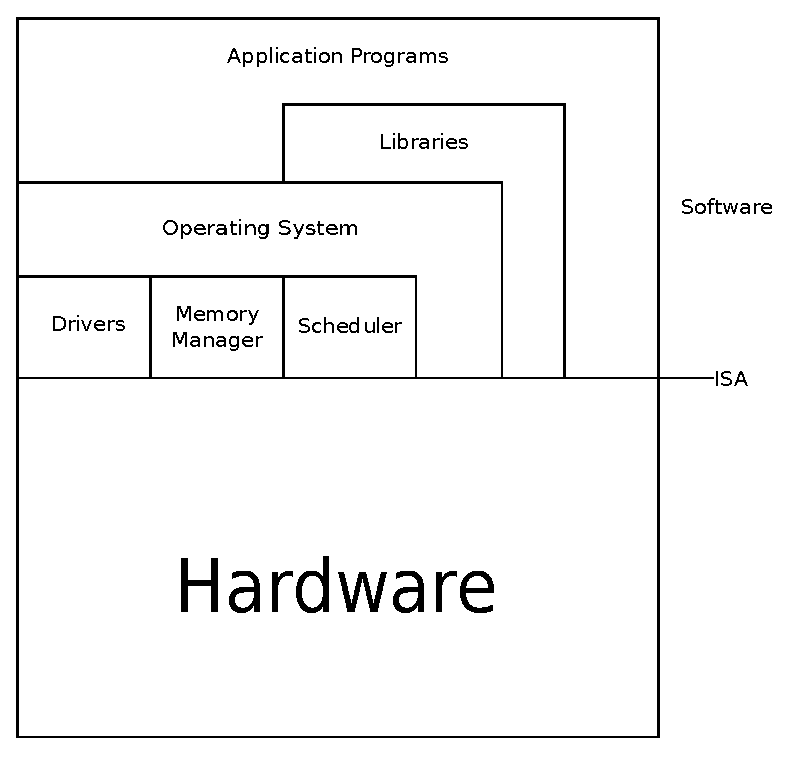
\includegraphics[width=0.35\textwidth]{Hauptteil/csa.eps}
\caption{Computer System Architektur nach~\cite{virtualmachines}}
\label{fig:mbs}
\end{figure}

Um nun mit den verschiedenen Geräten über eine Vielzahl von Schnittstellen kommunizieren
zu können, benötigt jedes Gerät einen eigenen Treiber. Dieser Treiber ist im Betriebssystem
als \emph{„Wissen“} hinterlegt und beinhaltet Information über das Gerät und dessen
Zugriffsmöglichkeiten.~\cite{treiber}\\

\textbf{Compiler}\\
Der Compiler ist ein Werkzeug, welches einen Quelltext, der in einer höheren Programmiersprache (C++, C, Java) geschrieben wurde, in Maschinenbefehle umsetzt.
 Damit der Prozessor diese Instruktionen ausführen kann, werden die lesbaren Programmierbefehle übersetzt. Nach dem so genannten Kompilieren steht das Programm zur Ausführung bereit.
Die Aufgaben des Compilers bestehen grundsätzlich aus drei Schritten:\cite{compiler}
\begin{enumerate}
  \item Lexikalische Analyse:
  	Der Compiler zerlegt die Wörter und Zeichen des Quelltextes in verschiedene Klassen. Dabei werden überflüssige oder fehlende Zeichen als Fehler erkannt und vom Compiler, je nach
  schwere des Verstoßes, als Warning oder Error ausgegeben.
  \item Parsing:
  	Es folgt die Prüfung des Codes auf syntaktische Korrektheit.
  \item Semantische Analyse: Der Quelltext wird auf Sinnhaftigkeit geprüft. Zum Beispiel ob Befehle wirklich die korrekten Parameter haben.
\end{enumerate}

Im Vergleich zum Interpreter gibt es folgende Vor- und Nachteile.

Vorteile:
\begin{itemize}
  \item effiziente Übersetzung in ausführbaren Code
  \item Optimierung des generierten Codes
\end{itemize}

Nachteile:
\begin{itemize}
  \item Kompilieren benötigt Zeit und Ressourcen
  \item Neu-Kompilierung nach Quelltextänderung
  \item Jede Programmiersprache benötigt einen eigenen Compiler
\end{itemize}

\begin{figure}[H]
\centering
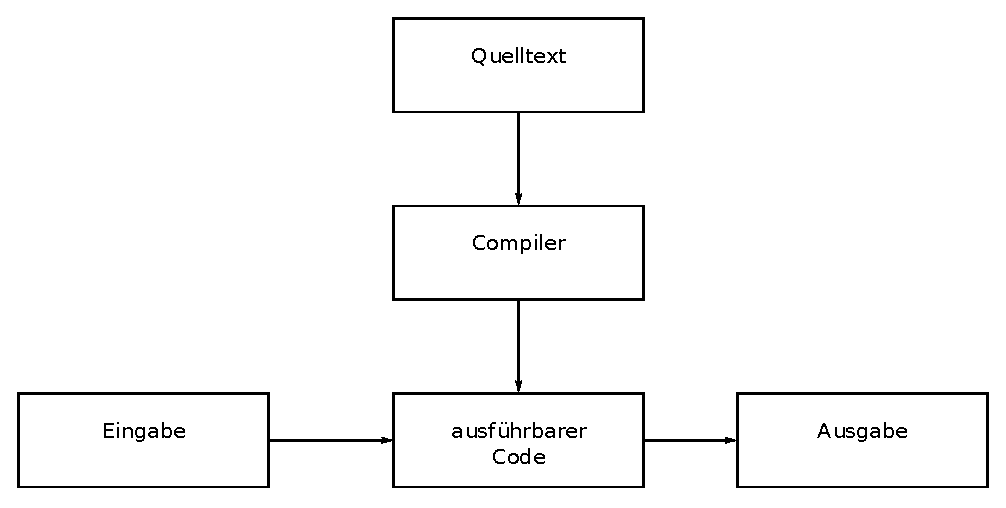
\includegraphics[width=0.8\textwidth]{Hauptteil/Compiler.eps}
\caption{Funktionsweise des Compilers}\label{fig:compiler}
\end{figure}

\textbf{Compiler-Modi}\\
Der im Kapitel zuvor beschriebene Compiler kann, je nach Zielsystem, in verschiedenen Modi betrieben werden. Hier bei ist der ausschlaggebende Punkt, ob auf dem System ein Betriebssystem ausgeführt werden soll oder nicht.\\

\begin{itemize}
  \item Non-OS mode: Programme ohne Zugriff auf Ein- bzw. Ausgabegeräte. Programme, welche in diesem Modus ausgeführt werden, haben keine periphere Unterstützung.
        Der Bare-Metal-Mode wird meistens genutzt, um \ac{isa}- und Cache-Regressionstests durchzuführen. Hierbei entscheidet der Rückgabewert des Programmes über Erfolg beziehungsweise Misserfolg
        des Tests. \emph{0} bedeutet Erfolg, Zahlen ungleich \emph{0} geben den jeweiligen Fehlercode an. Bare-Metal-kompilierte Programm laufen auf einem \ac{fpga} und in einer Simulation
        im Hintergrund. \\
        Um nun mit einem Bare-Metal-Programm eine Ausgabe zu erzeugen, müssen Bibliothkenen verwendet werden, welche die Art und Weise der Ausgabe beinhalten.\\

        \begin{figure}[H]
        \centering
        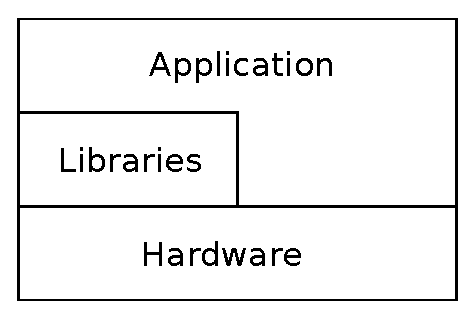
\includegraphics[width=0.3\textwidth]{Hauptteil/baremetal.eps}
        \caption{Grafische Darstellung der Non-OS-Architektur}\label{fig:baremetal}
        \end{figure}

  \item Linux mode: Benutzerprogramme mit Linux-Unterstützung. Mit Hilfe dieser Programme lassen sich Verhaltssimulationen auf dem \ac{fpga}-Board durchführen. Diese Programme
  erhalten Multi-Thread und Peripherie-Unterstützung vom Linux-Kernel\cite{lowrisc}\\

  \begin{figure}[H]
  \centering
  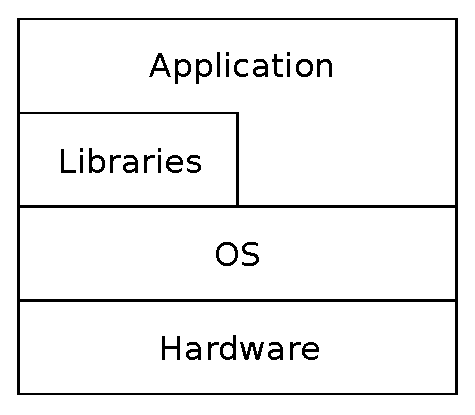
\includegraphics[width=0.3\textwidth]{Hauptteil/linuxmode.eps}
  \caption{Grafische Darstellung der Linux-Architektur}\label{fig:linuxmode}
  \end{figure}
\end{itemize}

\subsection{Hardware-Voraussetzung}\label{kap:hardwarevoraussetzung}

\textbf{Prozessor}\\
Die \ac{cpu} ist das sogenannte Gehirn des Computers. Sie ist für die Ausführung der Programme zuständig, welche im Hauptspeicher abgelegt sind. Dazu ruft sie nacheinander
Befehle ab, analysiert diese und führt sie anschließend aus. Um diese Aufgaben bewältigen zu können, besteht die \ac{cpu} im wesentlichen aus drei Komponenten, welche
in Abbildung~\ref{fig:cpu} grafisch dargestellt sind. Diese Komponenten sind über einen Bus miteinander verbunden, dessen Leitungen Adresse, Daten und Steuersignale übertragen. Mit Hilfe von externen Bussen lässt sich die \ac{cpu} mit dem Speicher, sowie Eingabe- und Ausgabegeräten
verbinden.~\cite{cache}
\begin{itemize}
  \item Das Steuerwerk (\ac{cu}) analysiert mit Hilfe des Instruktionsdecoders ein Maschinenenwort und übersetzt diese in eine Reihe von Steuersignalen, die den weiteren
        Ablauf der Befehlsabarbeitung beeinflussen. Somit übernimmt es die Aufgabe den Kontroll- und Datenfluss zu überwachen und den korrekten Datentransport sicherzustellen.~\cite{benchmark}
  \item Das Rechenwerk (\ac{alu}) führt Operationen aus, die für den jeweiligen Befehl notwendig sind, wie beispielsweise Addition oder Verknüpfungen~\cite{benchmark}
  \item Prozessorregister lassen sich in Universal- und Hilfsregister einteilen. Sie bieten die Möglichkeit, Zwischenergebnisse und Steuerinformationen aufzunehmen,
        welche sehr schnell gelesen und geschrieben werden können~\cite{benchmark}
\end{itemize}

\begin{figure}[H]
\centering
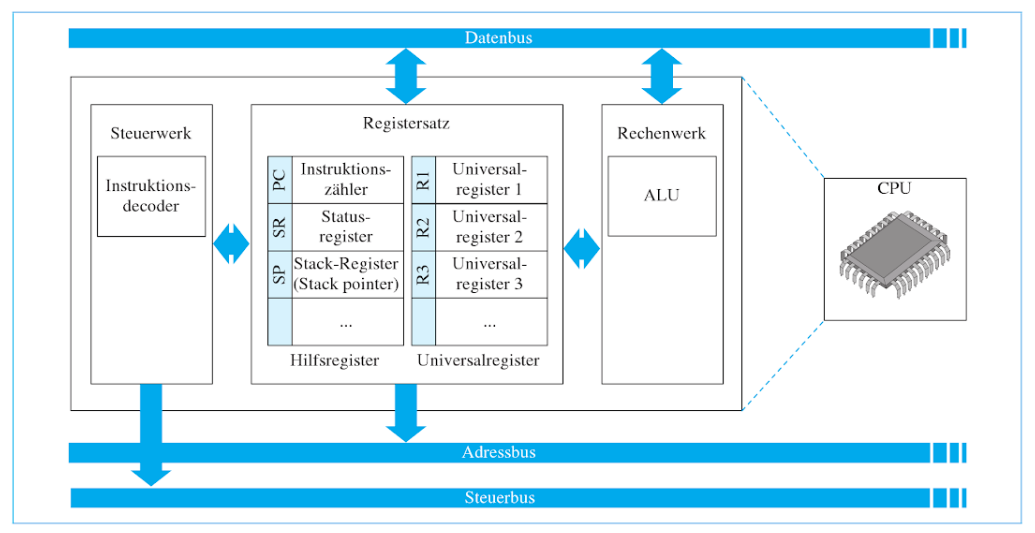
\includegraphics[width=0.95\textwidth]{Hauptteil/cpu.png}
\caption{Die innere Struktur eines Mikroprozessors~\cite{benchmark}}\label{fig:cpu}
\end{figure}


Das wichtigste Register ist der Befehlszähler (engl. Program Counter), welcher auf den nächsten Befehl zeigt, der zur Ausführung aufzurufen ist. Daneben
ist der Befehlsregister (engl. Instruction Register) ein wichtiger Bestandteil, da er den momentan ausgeführten Befehl aufnimmt.\\
Daraus ergibt sich zur Befehlsausführung eine Schrittfolge, die als Abrufen-Dekodieren-Ausführen-Zyklus (engl. Fetch-Decode-Execute Cycle) bezeichnet wird.~\cite{cache}
\begin{enumerate}
  \item Den nächsten Befehl aus dem Speicher in das Befehlsregister abrufen
  \item Den Programmzähler ändern, damit er auf den nächsten Befehl zeigt
  \item Den Typ des gerade eingelesenen Befehls bestimmen
  \item Falls der Befehl ein Speicherwort benötigt, dessen Position bestimmen
  \item Das Wort bei Bedarf in ein \ac{cpu}-Register abrufen
  \item Den Befehl ausführen
  \item Den Vorgang wiederholen, um nächsten Befehl auszuführen
\end{enumerate}

\textbf{Softcore-Prozessoren}\\
Ein SoftCore (engl. „Software-Kern“) ist ein Prozessor, Mikrocontroller oder ein Signalprozessor, welcher als virtuelle Einheit in einem \ac{fpga} oder \ac{asic} integriert wird.
Dies bietet die Möglichkeit einem digitalen Schaltungsdesign jeden beliebigen Prozessor hinzuzufügen.\\
Umgesetzt wird dieser Vorgang im \ac{fpga} durch reine Anwenderlogik,
welche dementsprechend konfiguriert werden muss.\\
Das typische Anwendungsgebiet eines SoftCores ist die Lösung von komplizierten Aufgaben, mit denen klassische „State Machines“ überfordert sind oder die Effektivität
 nicht mehr gegeben ist. Somit werden SoftCores oftmals nachträglich in bestehende Designs eingefügt, wenn deren Umfang sich extrem vergrößert hat.\cite{softcore}\\

\textbf{Vergleich SoftCores und HardCores}\\
Vergleicht man den SoftCore- mit dem HardCore-Prozessor, lassen sich folgende Aussagen treffen.

Vorteile:
\begin{itemize}
   \item Flexible Anwendung: Das \ac{fpga} kann bei Bedarf mit einem SoftCore versehen werden, jedoch wird nicht von vorneherein Platz für einen HardCore verschwendet, welcher
    dann letztendlich ungenutzt bleibt. Daraus ergeben sich deutliche Vorteile im Hinblick auf die Kosten.
    \item Konfigurierbarkeit: Beim SoftCore deutlich flexibler, da hier unter anderem die Größe der Datenpfade und die Anzahl der Zusatzmodule variiert werden kann.
 \end{itemize}


Nachteile:
\begin{itemize}
  \item SoftCores haben auf Grund ihrer Flexibilität einen deutlichen Geschwindigkeitsnachteil
\end{itemize}

% \subsection{Typen}\label{kap:typen}
% Es gibt eine große Anzahl verschiedener SoftCores. Diese unterscheiden sich aber maßgeblich in der Größe der Datenpfade.
% Somit wird unterschieden zwischen 8-,16- und 32-Bit Systemen.\cite{softcore}\\
%
% \textbf{8-Bit SoftCores}\\
% \begin{table}[H]
% \centering
% \begin{tabular}{|l|c|r|}
%   \hline
%   \textbf{Name} & \textbf{Quellcode} & \textbf{Hersteller}\\
%   \hline
%   LatticeMico8 & Verilog und VHDL & Lattice\\
%   \hline
%   PicoBlaze & VHDL & Xilinx\\
%   \hline
%   Proteus & VHDL & LogicSolutions\\
%   \hline
% \end{tabular}
%   \caption{8-Bit SoftCores nach ~\cite{softcore}}
%  \label{tab:8bitsysteme}
%   \end{table}
%
%   \textbf{16-Bit SoftCores}\\
%   \begin{table}[H]
%   \centering
%   \begin{tabular}{|l|c|r|}
%     \hline
%   \textbf{Name} & \textbf{Quellcode} & \textbf{Hersteller}\\
%     \hline
%     NEO430 & VHDL & neo430@GitHub\\
%     \hline
%     OpenMSP430 & Verilog & OpenCores\\
%     \hline
%     TG68 & VHDL & OpenCores\\
%     \hline
%   \end{tabular}
%     \caption{16-Bit SoftCores nach ~\cite{softcore}}
% \label{tab:16bitsysteme}
%     \end{table}
%
%     \textbf{32-Bit SoftCores}\\
%     \begin{table}[H]
%     \centering
%     \begin{tabular}{|l|c|r|}
%       \hline
%     \textbf{Name} & \textbf{Quellcode} & \textbf{Hersteller}\\
%       \hline
%       LEON & VHDL & Gaisler Research\\
%       \hline
%       Microblaze & Nein & Xilinx\\
%       \hline
%       OpenRISC & Verilog & OpenCores\\
%       \hline
%       NIOS II & Nein & Altera\\
%       \hline
%     \end{tabular}
%       \caption{8-Bit SoftCores nach~\cite{softcore}}
%      \label{tab:8bitsysteme}
%       \end{table}
%
%
%
%




\newpage

\textbf{Memory Management Unit}\\
Bei der \ac{mmu} handelt es sich um einen Hilfsbaustein des Betriebssystems, welcher die Speicherverwaltung des Arbeitsspeichers beschleunigt. Umgesetzt wird diese Verwaltung mit
Hilfe eines Verfahren, welches virtuelle Adressen auf physikalische Adressen abbildet. Der gesamte Speicher wird in einzelne Speicherbereiche unterteilt und die
\ac{mmu} überwacht die Einhaltung dieser Bereiche und unterbricht gegebenenfalls Instruktionen, die auf einen verbotenen
Bereich zugreifen wollen.\cite{itwissen}\\

\begin{figure}[H]
\centering
\includegraphics[width=0.8\textwidth]{Hauptteil/mmu.eps}
\caption{Blockschaltbild einer MMU}\label{fig:mmu}
\end{figure}


\textbf{Cache}\\
Eine der größten Herausforderungen im Computerdesign ist es, Speichersysteme zu schaffen, welche den Prozessoren mit Operanden mit einer Geschwindigkeit versorgt, mit der er arbeiten kann.
Moderne Prozessoren stellen höchste Ansprüche an ein Speichersystem, sowohl hinsichtlich der Latenzzeit, sowie hinsichtlich der Bandbreite. Diese beiden Aspekte stellen einen Konflikt dar. So führen
Methoden zur Steigerung der Bandbreite unmittelbar zur Erhöhung der Latenzzeit.
Ebenfalls wird es immer schwieriger ein Speichersystem zu realisieren, welches mit der steigenden Geschwindigkeit des Prozessors agieren kann.\\
Eine Lösung für dieses Problem sind die Caches. Ein Cache nimmt die zuletzt benutzten Speicherworte in einen kleinen, schnellen Speicher auf, sodass der erneute Zugriff darauf beschleunigt wird.
Somit verringert sich die effektive Speicherlatenz enorm, wenn sich ein ausreichend großer Anteil der benötigten Speicherworte im Cache befindet.\\
Ein Einsatz mehrerer Caches ermöglicht es, sowohl die Bandbreite, als auch die Latenzzeit zu verbessern. Für die grundlegende Verbesserung bietet sich der sogenannte Cache-Split an, bei
welchem der Instruktion und der Datencache getrennt werden. Darauf folgt, dass ein unabhängiges Einleiten von Speicheroperationen in verschiedenen Caches die Bandbreite des
Speichersystems quasi verdoppelt. In der praktischen Umsetzung besitzt jeder Port seinen eigenen Cache und jeder Cache kann unabhängig von anderen auf den Hauptspeicher zugreifen.\\
Als weitere Möglichkeit zur Leistungsverbesserung ist es in modernen Systemen üblich, einen Level-2-Cache zu nutzen. Dieser kann zwischen dem Befehls- und Daten-Cache, sowie dem Hauptspeicher
angesiedelt sein. Je nach Anforderung an das Speichersystem, können weitere Cache-Ebenen hinzugefügt werden. \\


\begin{figure}[H]
\centering
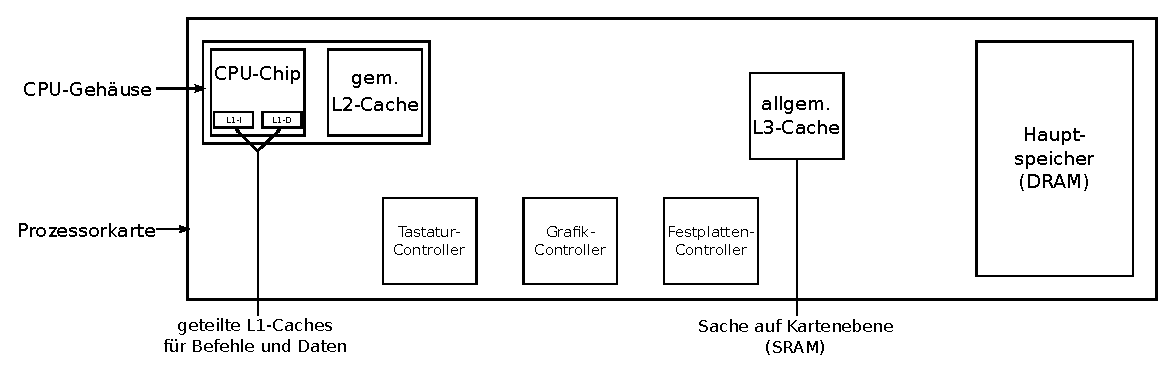
\includegraphics[width=1\textwidth]{Hauptteil/Cache.eps}
\caption{Ein System mit drei Cache-Ebenen nach~\cite{cache}}\label{fig:cache}
\end{figure}





Die Abbildung~\ref{fig:cache} zeigt ein klassisches System mit drei Cache-Ebenen. Diese Ebenen unterscheiden sich vorwiegend durch ihre Größe. So beinhaltet der \ac{cpu}-Cache einen kleinen Cache
in der Größenordnung von 16KB bis 64KB. Der Level-2-Cache, welcher neben dem \ac{cpu}-Chip angeordnet und mit einem Hochgeschwindigkeitspfad verbunden ist, besitzt üblicherweise eine Größe von
 512 KB bis 1 MB. Hierbei handelt es sich typischerweise um einen sogenannten \emph{unified} (gemeinsamen) Cache, welcher eine Mischung aus Daten und Befehlen beinhaltet. \\
 Die dritte Cache-Ebene besteht aus einigen Megabyte \ac{sram} und wird auf der Prozessorkarte angeordnet. Dieser \ac{sram} bietet einen enormen Vorteil in der Geschwindigkeit gegenüber dem
 Hauptspeicher (\ac{dram}). \\
 Eine Besonderheit der Caches ist, dass diese umfassend sind, das bedeutet, dass der gesamte Inhalt des L1-Caches im L2-Cache und der gesamte L2-Cache Inhalt im L3-Cache  enthalten ist.\\
 \newpage
Bei dem Prinzip der Adresslokalitäten bedienen sich Caches zwei verschiedenen Arten:\\

\begin{itemize}
  \item örtliche Lokalität (Spartial Locality): Beschreibt die Beobachtung, dass auf Speicherstellen mit 	Adressen, die einer kürzlich angesprochenen Speicherstelle numerisch ähnlich sind, in der
   	nächsten Zeit wahrscheinlich zugegriffen wird. Dadurch werden mehr Daten eingelesen als 	angefordert und damit die Annahme getätigt, dass Anforderungen vorausgesagt werden 	können.
  \item zeitliche Lokalität (Temporal Locality): Auf Speicherstellen, auf die kürzlich zugegriffen wurde, 	wird erneut zugegriffen.  Als praktisches Beispiel gelten hier Funktionen innerhalb
        einer Schleife. Diese Art der Lokalität wird oft zur Fehlerbehebung genutzt,  wenn es zu Cache-	Zugriffsfehlern kommt.\\
\end{itemize}

Grundsätzlich basieren Caches auf dem Prinzip, dass der Hauptspeicher in Blöcke unterteilt wird, welche eine feste Größe besitzen. Dies sind die sogenannten Cache-Zeilen (Cache-Lines).
Diese bestehen aus aufeinander folgenden Bytes in einer Größenordnung von 4 bis 64 Bytes. Bei Speicherzugriffen wird geprüft, ob sich das angeforderte Wort im Cache befindet und direkt
vom Prozessor verwendet werden kann. Ist dies nicht der Fall, wird ein Zeileneintrag aus dem Cache entfernt und die benötigte Zeile aus dem Hauptspeicher geladen. \\
Es gibt zwei grundlegende Arten des Caches. Die einfachste Art Cache zu realisieren, ist die Form des direkt abbildenden Caches. Dabei kann jeder Eintrag, beziehungsweise Zeile, genau
eine Cache-Zeile aus dem Hauptspeicher aufnehmen. Besitzt der Cache eine Zeilengröße von 32 Bytes, nimmt der Cache 64 KB auf. Daraus lässt sich schlussfolgern, dass eine bestimmtes
Wort an genau einer Stelle im Cache liegen kann. Ist das Wort nicht an dieser Adresse zu finden, ist es auch nicht im Cache enthalten. \\

Diese Adresse lässt sich in vier Komponenten zerlegen:
\begin{itemize}
  \item TAG\@: Entspricht den Tag-Bits, welche in einem Cache-Eintrag gespeichert sind
  \item LINE\@: Beinhaltet die Information, in welchem Cache-Eintrag sich die Daten befinden, falls vorhanden
  \item WORD\@: Gibt an, welches Wort innerhalb einer Zeile angefordert wurde
  \item BYTE\@: Wird in Ausnahmefällen genutzt, um einzelne Bytes anzufordern
\end{itemize}





Mit diesen Eigenschaften stellen die direkt abbildenden Caches den am häufigsten verwendeten Cache-Typen dar, weil diese effektiv arbeiten und Kollisionen, bei zum Beispiel identischer LINE,
selten, beziehungsweise gar nicht vorkommen. \\
Das Problem der Speicherkollisionen lässt sich wiederum mit der Verwendung von zwei oder mehr Zeilen pro Cache-Eintrag lösen. Dieser Typ mit \emph{n}-möglichen Einträgen für jede Adresse,
 wird als n-fach mengen-assoziativen Caches (engl. N-way set-associativ Cache) bezeichnet.Im Vergleich zu dem beschriebenden direkt abbildenden Cache ist der mengen-assoziative Cache
 komplizierter, da sich zwar der korrekte Cache-Ebene aus der Speicheradresse berechnen lässt, hierfür jedoch \emph{n} Einträge geprüft werden müssen. Somit ergibt sich ein Nachteil
 was Schnelligkeit anbelangt, jedoch zeigt die Erfahrung, dass sich der Mehraufwand lohnt und 2-, sowie 4-fach Caches gute Leistungen erzielen können.~\cite{cache} \\


 \textbf{Interrupt}\\
 Neben der \ac{cpu} und dem Datenspeicher haben die meisten Computersysteme Peripherie. Es handelt sich dabei um verbaute oder um an Schnittstellen angeschlossene Geräte.
 Damit die \ac{cpu} die Nachricht erhält, dass Daten an solch einer Schnittstelle beziehungsweise Verbindung anliegen, muss es eine Möglichkeit geben den Prozessor zu
 unterbrechen. Hier gibt es die Art des sogenannten Polling, bei dem der Prozessor alle vorhandenen Eingabegeräte zyklisch abfragt. Ein effektiveres Verfahren ist die
 Unterbrechungsanforderung (Interrupt), welche eintritt, wenn Daten anliegen. \\
 Sobald ein Gerät Daten zur Weiterverarbeitung besitzt, wird ein \ac{irq} auf der dafür vorgesehenen Interrupt-Leitung gesendet. Daraufhin unterbricht der Prozessor
 seine Arbeit und verarbeitet die Daten des Gerätes.\cite{irq}\\

 \begin{figure}[H]
 \centering
 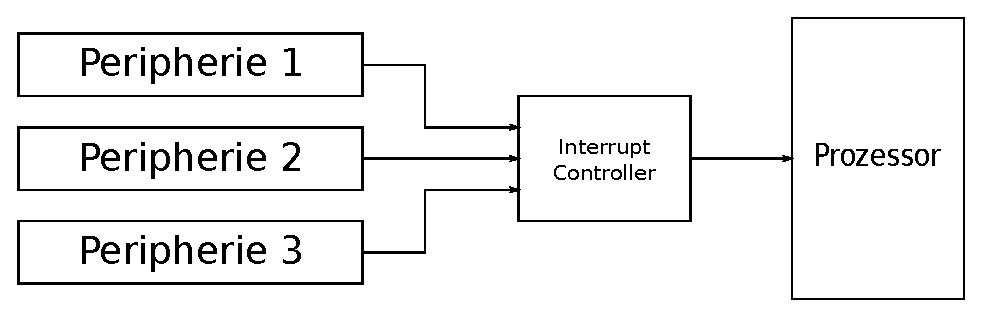
\includegraphics[width=0.8\textwidth]{Hauptteil/irq.eps}
 \caption{Interrupt-Controller}\label{fig:irq}
 \end{figure}

\newpage

 %
 % \textbf{Peripherie}\\
 % Ein Peripheriegerät kann einer Hardware hinzugefügt werden, um die Fähigkeiten zu erweitern. Diese Geräte sind optional und dienen zur Ein- und Ausgabe von Daten.\\

\textbf{UART}\\
Um mit Peripheriegeräten zu kommunizieren, kann \ac{uart} als serielle Schnittstelle genutzt werden.
Bei dieser Art der Kommunikation werden serielle Daten zwischen dem Board (\emph{Master})
und dem Empfänger (\emph{Slave}) ausgetauscht. \\
Dabei spielen die TxD und die RxD-Datenleitungen
eine wichtige Rolle, da der Datenaustausch über diese Leitungen realisiert wird.\\
Im Gegensatz, zum Beispiel, zu einer \ac{spi}-Schnittstelle, wird kein Clock-Signal
übertragen um Daten zu validieren. Des Weiteren wird die Verbindung mit einer definierten
Geschwindigkeit realisiert, der sogenannten \emph{Baudrate}.~\cite{uartpdf} \\
Die Baudrate bezeichnet dabei die Anzahl der Bits, welche pro Sekunde übertragen werden.
\ac{uart} konvertiert die Bytes in serielle Bits, überträgt diese über eine einzelne Leitung
und liest die zugehörigen Start- und Stop-Bits aus.\\
Das sogenannte \emph{Character}(Zeichen) besteht aus einer konfigurierbaren Anzahl an Datenbits (in den meisten
Fällen 7 oder 8), aus einem \emph{low-level} Start-Bit, einem optionalen Parity-Bit und einem
oder mehreren logischen \emph{high-level} Stop-Bits.\\
Das Start-Bit teilt dem Receiver mit, dass ein neues \emph{Character} empfangen wird.
Die nächsten Bits, je nachdem wie viele Daten-Bits vorher konfiguriert wurden, stellen
dann den Inhalt des \emph{Character} dar. Darauf folgt das optionale Parity-Bit,
welches anzeigt, ob die Anzahl der mit '\emph{1}' belegten Daten-Bits gerade oder
ungerade ist. Am Ende der Folge stehen dann entweder ein oder zwei  \emph{high-level } Stop-Bits,
welche dem Receiver eindeutig signalisieren, dass die Übertragung vollständig ist. Dadurch,
dass das Start-Bit \emph{high-level} (1) und das Stop-Bit \emph{low-level} (0) ist,
ist immer eine klare Abgrenzung zwischen dem derzeitigen und dem folgenden \emph{Character} möglich.\\

Die Datenübertragung lässt sich nach~\ref{fig:uart} darstellen.\\

\begin{figure}[h!]
\centering
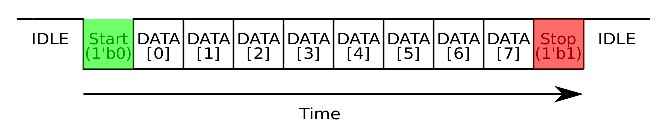
\includegraphics[width=0.8\textwidth]{Hauptteil/uart.eps}
\caption{Datenübertragung per \ac{uart}(8n1) }
\label{fig:uart}
\end{figure}

\newpage
\textbf{Timer}\\
Ein weiterer essenzieller Teil zur Ausführung eines Betriebssystems, wie zum Beispiel Linux, ist der Timer. Dieser hilft dem Betriebssystem dabei, das so genannte Scheduling
durchzuführen. Hierbei wird mit Hilfe von \emph{Timer}-gesteuerten Interrupts dafür gesorgt, dass Nutzerprogramme, welche sich in der Ausführung befinden, unterbrochen werden und
in den Betriebssystem-Modus geschaltet wird. Nun kann das Betriebssystem die anstehenden Prozesse neu planen.\\










\section{Benchmark}\label{kap:benchmark}
Geht es um die Leistungsfeststellung eines Systems täuschen oft Zahlen der Hersteller die potentiellen Käufer. Im Falle der \ac{cpu} ist es neben der Anzahl der Prozessorkerne
 fast immer die Taktfrequenz, welche angegeben wird.
Die Taktfrequenz hat zweifelsohne einen großen Einfluss auf die Geschwindigkeit einer \ac{cpu}, jedoch ist diese Zahl ohne weitere Informationen, wie zum Beispiel die
Mächtigkeit des Befehlssatzes, in ihrer Aussagekraft eingeschränkt. Dies gilt selbst, wenn beide Prozessoren die gleiche Instruktionsstruktur aufweisen, da es bei der
internen Implementierung zu erheblichen Unterschieden kommen kann. \\
Um hier einen aussagekräftigen Vergleich zu erzielen, wurden verschiedene Maßzahlen eingeführt, wie beispielsweise \ac{mips}, der \ac{ipc}-Wert oder ac{mflops}. Diese
 Zahlen bieten zwar eine genaue Auskunft über bestimmte Architekturaspekte, ein Rückschluss auf die wirklich erreichbare Geschwindigkeit beim Ausführen eines Programmes
 unter realen Bedingungen ist nur bedingt möglich. \\
So wurde festgelegt, dass die Leistung unter Ausführung fest definierter, als Benchmark bezeichneter Referenzprogramme ermittelt wird. Als Maß gilt entweder die gemessene
 Laufzeit zwischen Start und Ende des Programms oder die Anzahl der Operationen, die in einer genormten Zeiteinheit ausgeführt werden. Damit diese Ergebnisse aussagekräftig
 und nicht verfälscht sind, müssen die verschiedenen Benchmark-Programme unter reproduzierbaren Bedingungen ausgeführt werden. Dies wird bei heutigen Betriebssystemen zunehmend
  schwieriger, da selbst Dienstprozesse die Messung erheblich stören können.~\cite{benchmark}

\subsection{Dhrystone}\label{kap:dhrystone}
Der Dhrystone-Benchmark wurde 1984 von Reinhold P. Weicker entwickelt. Die Besonderheit dieses Benchmark ist, dass sie vollständig
ohne Gleitkommaoperationen auskommt, was im Fall dieser Arbeit enorm wichtig war, weil nicht bei allen Systemen eine \ac{fpu} vorhanden ist.
Die ursprüngliche Version basierte noch auf dem Ada-Code, heutzutage wird die Leistungsmessung fast ausschließlich durch C-Implementierungen
 realisiert. Die Benchmark beinhaltet eine Mischung aus Befehlen, welche typischerweise von Compilern erzeugt werden. Insgesamt handelt es sich
 um rund 100 Befehle, die aus einfachen Zuweisungen und Fallunterscheidungen, sowie Schleifen, Sprüngen und Funktionsaufrufen bestehen.
  Diese Dhrystone-Befehle werden durchgängig in Form einer Schleife ausgeführt, wobei die Anzahl der Durchgänge vor der Ausführung vom
  Nutzer festgelegt werden kann. Im Endeffekt entspricht die Leistung des Prozessors der Anzahl der in einer Sekunde durchgeführten Schleifendurchläufe.
  Das Ergebnis der Benchmark wird als \emph{Dhrystones per Second} angegeben. Um diesen Wert nun in die Einheit \ac{dmips} umzurechnen wird der Faktor 1757 benötigt. Dieser Skalierungsfaktor
  stammt von einer VAX 11/780, auf welcher die Dhrystone-Benchmark ausgeführt wurde und ein Wert von 1757 erreichte und somit als 1-\ac{mips}-Maschine angesehen wurde. Also ergibt sich der
  \ac{dmips}-Wert aus der Division des \emph{Dhrystones per Second} und dem Skalierungsfaktor.~\cite{benchmark}

  \subsection{Coremark}\label{kap:coremark}
  Der CoreMark von \ac{eembc} ist ein Benchmark, der die Leistung von \ac{mcu} und \ac{cpu} misst, die in eingebetteten Systemen verwendet werden.
   Coremark enthält Implementierungen der folgenden Algorithmen: Listenverarbeitung (Suchen und Sortieren),
    Matrixmanipulation (gemeinsame Matrixoperationen), Zustandsmaschine (prüft, ob ein Eingabestream gültige Zahlen enthält) und \ac{crc} (zyklische Redundanzprüfung).
    Es kann auf Geräten von 8-Bit-Mikrocontrollern bis zu 64-Bit-Mikroprozessoren ausgeführt werden.
  Der \ac{crc}-Algorithmus erfüllt eine Doppelfunktion; Es bietet eine Arbeitslast, die häufig in eingebetteten Anwendungen zu finden ist
  und gewährleistet den korrekten Betrieb der CoreMark-Benchmarks, die im Wesentlichen einen Mechanismus zur Selbstüberprüfung bereitstellt.
   Insbesondere wird zur Überprüfung der korrekten Operation ein 16-Bit-\ac{crc} anhand der Daten ausgeführt, die in Elementen der verknüpften Liste enthalten sind.\\
  Um sicherzustellen, dass der Compiler die Ergebnisse zur Kompilierungszeit nicht vorberechnen kann, leitet jede Operation im Benchmark einen Wert ab,
  der zur Kompilierungszeit nicht verfügbar ist. Darüber hinaus ist jeder Code, der innerhalb des zeitgesteuerten Teils der Benchmarks verwendet wird,
  Teil des Benchmarks selbst (keine Bibliotheksaufrufe).
  Die CoreMark-Benchmark überprüft Pipeline-Operationen, Speicher (inklusive Cache, falls vorhanden), sowie den Zugriff und das Handling von Integer-Operationen.
  Wenn die Coremark auf einer \ac{mcu} oder \ac{cpu} ausgeführt wird, ergibt sich ein so genannter Score, welcher einen schnellen Vergleich zwischen verschiedenen Prozessoren ermöglicht.~\cite{coremark}


  Grundlegende Eigenschaften:
\begin{itemize}
  \item Geschrieben in kleinem und leicht verständlichen C-Code
  \item Bietet eine realistische Mischung aus Lese- und Schreiboperationen, sowie Ganzzahl- und Steueroperationen
  \item Besteht aus mehreren Algorithmen, die häufig verwendet werden
  \item funktioniert auch für Multicore-Systeme, in dem mehrere Instanzen des CoreMark gebildet werden
  \item Die Ergebnisse der bereits getesteten Systeme werden auf der Seite des Herstellers veröffentlicht.
\end{itemize}

%
% \subsection{SPEC CPU2017}\label{kap:spec}
% SPEC CPU2017 ist ein Software-Benchmark-Produkt der \ac{spec}, einer Non-Profit-Gruppe, zu der Computerhersteller,
% Systemintegratoren, Universitäten, Forschungsorganisationen, Verlage und Berater aus der ganzen Welt gehören. Es wurde entwickelt
% um Leistungsmessungen bereitzustellen, mit denen rechenintensive Arbeitslasten auf verschiedenen Computersystemen verglichen werden können.\\
%
% Im neuen SPEC CPU 2017 sind vier Suiten enhalten:\\
% \begin{itemize}
% \item SPECspeed 2017 Integer
% \item SPECrate 2017 Integer
% \item SPECspeed 2017 Floating Point
% \item SPECrate 2017 Floating Point
% \end{itemize}
%
% Wie der Name schon andeutet, messen die beiden \emph{Speed}-Varianten die Zeit bei Gleitkomma- und Integer-Berechnungen. Die \emph{Rate}-Messungen hingegen, ermitteln den Durchsatz. Da die vier Suiten
% noch einmal in verschiedenen Tests unterteilt sind, besteht das Paket am Ende aus 43 einzelnen Testmöglichkeiten. Beispiele für Variationen die der Integer-Bereich mitbringt sind: \\
% \begin{itemize}
% \item \ac{gnu}-Compiler
% \item Perl-Interpreter
% \item Video-Kompression
% \item diversie AI-Berechnungen
% \end{itemize}
%
%
% Im Bereich der Gleitkomma-Benchmarks sind Anwedungen zu finden, wie: \\
% \begin{itemize}
% \item 3D-Rendering
% \item Fluid- und Moleküldynamik
% \item optische Tomografie
% \item Ray-Tracing
% \end{itemize}
% Mit dieser großen Anzahl an Benchmarks möchte SPEC einen Test anbieten, der aktuelle, sowie zukünftige \ac{cpu} aussagekräftig und vergleichbar misst.~\cite{spec}

\subsection{Ramspeed}\label{kap:ramspeed}
RAMspeed ist ein kostenloses Open-Source-Dienstprogramm, welches zu Messung der Cache- und Speicherleistung von Computersystemen genutzt wird. Dabei bietet die Software bis zu 18 verschiedene
Benchmarks für verschiedene Maschinen wie zum Beispiel \emph{i386} oder \emph{amd64}. Um dabei ein hohes Maß an Portabilität zu bieten, wurde diese Benchmark vollständig in der Programmiersprache
C geschrieben. Das Softwarepaket besteht aus zwei Hauptkomponenten:~\cite{ramspeed}
\begin{itemize}
  \item INTmark und FLOATmark: Diese messen die maximal mögliche Leistung des Caches und des Speichers beim Lesen beziehungsweise Schreiben bestimmter Datenblöcke. Dies geschieht in der Größenordnung ab 1 Kb und
                               verdoppelt sich jeweils in den nachfolgenden Messungen. Um die beste Performance zu erriechen sind alle Datenströme linear. Somit ermöglicht diese Benchmark die
                               tatsächliche Bandbreite eines Systems zu bestimmen.
  \item INTmem und FLOATmem: Hierbei handelt es sich um synthetische Simulationen, welche aus vier Untertests bestehen (Kopieren, Skalieren, Addieren, Triade). Diese verschiedenen Tests werden
                             genutzt um unterschiedliche Aspekte der Speicherleistung zu messen. Diese Benchmarks sind sehr empfindlich gegenüber Speicher-Latenzzeiten jeglicher Art.
\end{itemize}

Die vier Untertests lassen sich wie folgt näher beschreiben:
\begin{itemize}
  \item Kopieren: Die einfachste Methode, welche Daten von einem Speicherort zu einem anderen kopiert. (A = B)
  \item Skalieren: Dieser Test modifiziert die Daten vor dem Schreiben mit einem konstanten Wert. (A = m * B)
  \item Addieren: Hierbei werden Daten von zwei verschiedenen Speicherorten gelesen, miteinander addiert und letztendlich an einen dritten Speicherort geschrieben. (A = B + C)
  \item Triade: Bei dieser Operation handelt es sich um eine Zusammenführung der Addition und der Skalierung. Daten werden von einem Speicherort gelesen, skaliert und mit Daten eines zweiten Speicherortes
                addiert. Dieser Wert wird nun an einen weiteren Speicherort geschrieben. (A = m * B + C)
\end{itemize}

Die Anzahl von Gigabyte pro Durchlauf wurden in dieser Arbeit auf dem Wert \emph{1} gesetzt.

%
% \subsection{Device Tree}\label{kap:devicetree}
%
%
% Der \emph{Device-Tree} beinhaltet
% Informationen, welche dem Kernel bei dem Bootvorgang helfen. Da das System angeschlossene Geräte nicht automatisch erkennen
% und die dazu passenden Treiber laden kann, geschieht das in dieser \emph{.dts}-Datei. Durch das Kompilieren wird daraus
% der sogennante \emph{Device} \emph{Tree} \emph{Blob}. Dieser wird zusammen mit dem Kernel vom Bootloader geladen und im
% Hauptspeicher abgelegt. Im Anschluss daran wird daraus eine Baumstruktur. In dieser sind die Geräte als Knoten angelegt
% und es werden Informationen zu den dazugehörigen Treiber hinterlegt, welche dem Betriebssystem zur Verfügung gestellt werden.
% Die Verbindung zwischen Device-Tree und dem Treiber wird über eine
% eindeutige Identifikation per \emph{Compatible} festgelegt.
%
%
% \subsection{Buildroot}\label{kap:buildroot}
%
% \emph{Buildroot} ist ein Tool, welches das Erstellen eines kompletten Linux-Systems per
% \emph{Cross-Compiling} für eingebettete Systeme vereinfacht und automatisiert.  Neben dem
% \emph{cross-compiled} Toolchain können ebenfalls das \emph{Root}-Dateisystem, ein \emph{Linux-Kernel-Image}
% und ein \emph{Bootloader} für das Zielsystem erstellt werden.  In einem Konfigurationsprogramm lassen sich vor der
% Erstellung sämtliche Optionen und Erweiterungen ab- beziehungsweise anwählen. \\
% Das Tool wird größtenteils dafür genutzt, um die Systeme für andere Prozessoren, außer die klassischen x86-Prozessoren,
% zu erstellen, wie zum Beispiel \ac{arm}-Prozessoren.\cite{buildroot}\\
%
% \textbf{Toolchain}\\
%
% Bei der \emph{Toolchain} handelt es sich um eine Reihe von Tools zum Erstellen und Debuggen von Code für eine Zielarchitektur. Des Weiteren beinhaltet sie einen Compiler, einen Linker,
%  sowie verschiedene Bibliotheken.\\
%  Die Toolchain ist essenziell, um die drei weiteren Elemente eines eingebetteten Systems zu generieren: den Bootloader, den Kernel und das Root-Dateisystem. \\
%  Hierbei wird im wesentlichen zwischen zwei \emph{Toolchain}-Arten differenziert:
%  \begin{enumerate}
%    \item Die interne Toolchain: Die \emph{Toolchain} wird aus einer Quelle heraus vom \emph{Buildroot} generiert
%    \item die externe Toolchain: Es wird eine bereits vorhandene \emph{Toolchain} verwendet
%  \end{enumerate}
%
% Das Generieren einer eigenen \emph{Toolchain} benötigt entsprechend mehr Zeit und verlängert den ganzen Kompiliervorgang, bietet jedoch deutlich mehr Konfigurationsmöglichkeiten
% im Vergleich zu bereits vorhandenen \emph{Toolchains}.\\
%
% \textbf{Kernel}\\
%
% Der \emph{Kernel}, welcher bereits in Kapitel~\ref{kap:linux} beschrieben wurde, kann ebenfalls durch \emph{Buildroot} konfiguriert und erzeugt werden.\\
% Dieser steuert alle Prozessor-und Speicherzugriffe, unterhält die wichtigsten Treiber und greift direkt auf die Hardware zu. Dadurch, dass er die unterste Schicht des Systems beschreibt,
% ist er die Basis in der Kommunikation zwischen Hard- und Software.\\
% Zu seinen Aufgaben gehören neben der parallelen Verarbeitung verschiedener Aufgaben, auch die Einhaltung zeitkritischer Grenzen, sowie die Offenheit für unterschiedlichste Anwendungen
% und Erweiterungen. Im Falle des Linux-Systems gilt der Kernel als Vermittler im System, so ist die grafische Oberfläche komplett unabhängig vom Linux-Kernel.\cite{datacenter}\\
%
% \textbf{Root-Dateisystem}\\
%
% Der Kernel enthält keine Programme oder Dämonen, die das System an sich nutzbar machen. Hierfür ist das \emph{Root-Dateisystem} zuständig.\\
% Wichtige Inhalte sind:
% \begin{itemize}
%   \item init-Dämon: Startet Dämonen, Systemeinstellungen sowie Login-Programme
%   \item System-Konfiguration
%   \item Device-Nodes
%   \item Bibliotheken und Kernel-Module
% \end{itemize}
%
% Für die Zusammenstellung dieses Dateisystem kann \emph{Buildroot} verwendet werden, wodurch \emph{BusyBox} sowie weitere Programmpakete integriert werden.\cite{elektronikpraxis}\\
%
% \textbf{Bootloader}\\
%
% Der Bootloader, auch Boot Manager genannt, ist ein Programm, dessen Aufgabe es ist, das Betriebssystem in den Arbeitsspeicher zu laden. In diesem Fall ist er dafür verantwortlich,
% den Kernel mit den gewünschten Parametern zu laden und den Speicher zu initialisieren, bevor der eigentliche Boot-Prozess startet.\cite{searchdatacenter}\\
%
% \textbf{BusyBox}\\
%
% BusyBox kombiniert winzige Versionen vieler gängiger UNIX-Dienstprogramme in einer einzigen kleinen ausführbaren Datei.
% Es bietet Ersatz für die meisten Dienstprogramme, die normalerweise in GNU fileutils, Shellutils zu finden sind.
% Die Dienstprogramme in BusyBox haben im Allgemeinen weniger Optionen als ihre voll ausgestatteten GNU-Gegenstücke, welche jedoch die erwartete Funktionalität bieten und vom Verhalten sehr ähnlich sind.
% Ebenfalls bietet die BusyBox eine ziemlich vollständige Umgebung für eingebettete Systeme.\\
% BusyBox wurde größenoptimiert und für begrenzte Ressourcen geschrieben.
% Es ist auch extrem modular, sodass Befehle (oder Funktionen) zur Kompilierzeit ein- und ausgeschlossen werden können.
% Dies erleichtert die schnelle Anpassung der eingebetteten Systeme.\cite{busybox}\\
%

\chapter{Messergebnisse}\label{kap:ergebnisse}
Die Bewertung der Leistungsfähigkeit bestehender Soft-Cores stellt eine große Herausforderung für den Entwicklar dar, um den effizientesten und geeignetsten Soft-Core
für eine bestimmte Anwendung auszuwählen. Im Kapitel~\ref{kap:grundlagen} wurden bereits Soft-Cores, das Board, sowie die einzelnen Benchmarks näher erkläutert. Im folgenden Kapitel
soll nun ein Überblick über Soft-Core-Prozessoren gegeben werden, welche in eingebetteten System verwendet werden. \\
In dieser Arbeit wurden verschiedene Open-Source-, kommerzielle, sowie das unveröffentlichte System der Professur für Technische Informatik an der Helmut-Schmidt-Universität verglichen.
Dabei werden die verschiedenen Soft-Cores vorher nahezu identischen konfiguriert, um eine bessere Vergleichbarkeit herzustellen. Evaluiert wird bei den verwendeten Soft-Cores
die Auswirkung auf die gesamte Ausführungszeit und den \ac{fpga}-Flächenverbrauch. Um einen möglich aussagekräftigen Vergleich zu erzielen, ist es nötig die System nahezu identisch zu
konfigurieren. Dazu zählt vor allem die Entscheidung, alle Prozessoren als Single-Core zu konfigurieren, da das erstellen der Multi-Core-Prozessoren nicht bei allen Systemen ohne Weiteres
realisierbar war. Die übrigen Anforderungen an die Systeme sind in einem der nachfolgenden Kapitel angegeben.\\

\section{Verfügbare Soft-Core Prozessoren im Überblick}\label{kap:überblick}
Soft-Core Prozessoren werden häufig zur Ausführung eingebetteter Anwendungen eingesetzt, da sie wesentliche Vorteile im Hinblick auf Kosteneffizienz und Portabilität für verschiedene Systeme
beiten. So kann es bei der Auswahl durchaus schwierig sein den optimalen Prozessor auszuwählen. Einen Vergleich bietet die Tablle~\ref{tab:features}, in welcher sämtliche Eigenschaften
der Prozessoren aufgeführt sind.\\

\subsection{Microblaze}\label{kap:Microblaze}


Der Microblaze SoftCore von Xilinx ist eine 32-Bit RISC Harvard Architektur mit einem umfangreichen Befehlssatz. Aufgrund dieser RISC-Architektur
 wurde der Microblaze vor allem für einfache und zuverlässige eingebettete Systeme entwickelt und in diesen als zentraler Knoten beziehungsweise Hauptsteuereinheit
genutzt, da er über eine hohe Leistungsfähigkeit verfügt.

Konfiguriert wurde das System mit folgender Voreinstellung:~\cite{microblaze}\\
        \begin{itemize}
          \item \ac{spi} Controller
          \item I2C-Controller
          \item \ac{uart}
          \item Interrupt-Controller
          \item  Timer
          \item Instruktionscache
          \item \ac{mpu}
          \item Datencache
          \item DDR-Controller
          \item 32-Bit-Prozessorkern
          \item \ac{mmu}
          \item Ethernet-Controller
        \end{itemize}

Durch diese Konfiguration lassen sich folgende Schlüsselfähigkeiten des Systems ableiten:\\
\begin{itemize}
  \item 32 mal 32-Bit-\emph{General-Purpose}-Register
  \item 32-Bit-Befehlswort mit drei Operanden und zwei Adressierungsmodi
  \item 32-Bit-Adressbus, erweiterbar auf 64-Bit
  \item Optionale \ac{fpu}
  \item \ac{axi}4-Interface
  \item Verschiedene Zustandsmodi (Sleep, Hibernate, Suspend Mode/Instrctions)
  \item Unterstützt entweder \ac{plb}- oder \ac{axi}-Schnittstellen
  \item Big-Endian / Little-Endian Unterstützung
  \item Optionale \ac{mmu}, sowie separate, konfigurierbare Daten- und Instruktionscaches
\end{itemize}



\begin{figure}[H]
\centering
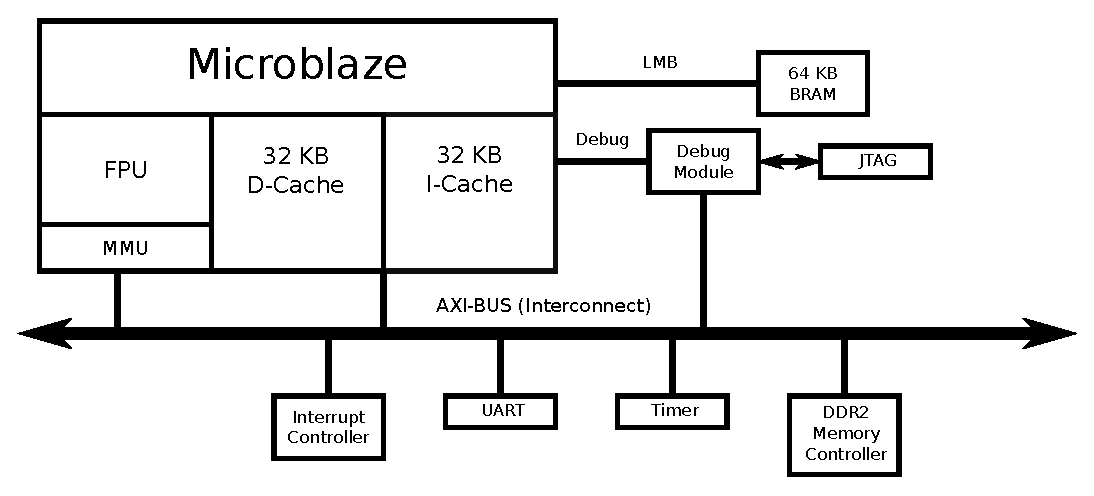
\includegraphics[width=1\textwidth]{Hauptteil/microblaze.eps}
\caption{\ac{soc}-Design des Microblaze nach~\cite{comparison}}
\label{fig:microblaze}
\end{figure}

Hierbei lässt sich erkennen, dass der Prozessor über den \ac{lmb} auf den On-Chip-Speicher zugreifen kann. Ist ein Zugriff auf externen Speicher erforderlich,
geschieht das über den \ac{plb}, an welchen weitere Peripheriegeräte angebunden sind. An diesen \ac{plb} ist ebenfalls der Timer angeschlossen, welcher das System mit einem Takt von
100 MHz taktet. Die Leistung des Microblaze kann gesteigert werden, indem das System um weitere Komponenten wie zum Beispiel \ac{fpu} oder \ac{bs} ergänzt wird.\\
\newpage
Die Leistung des Microblaze, basierend auf der Vivado-Version 2017.4, ist wie folgt angegeben:~\cite{microblaze}\\

\begin{figure}[H]
\centering
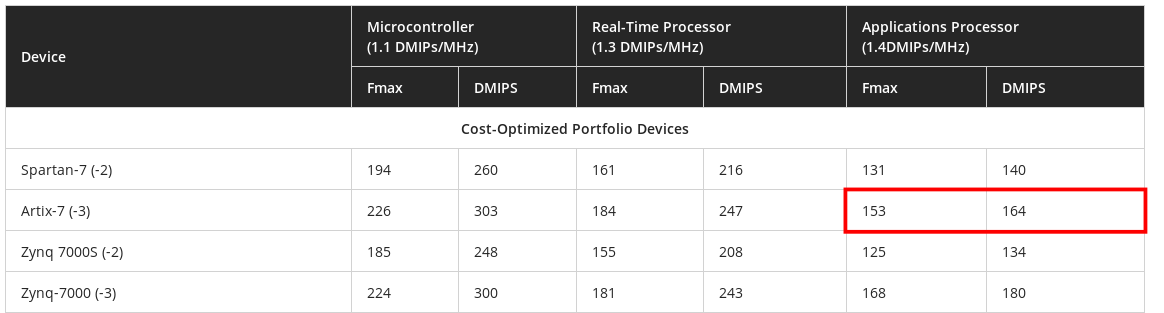
\includegraphics[width=0.7\textwidth]{Hauptteil/microblazeleistung.png}
\caption{Microblaze Performance Metrics: Basierend auf Vivado 2017.4 nach~\cite{microblaze}}
\label{fig:microblazeleistung}
\end{figure}

In der Abbildung~\ref{fig:microblazeleistung} sind die, für diese Arbeit, relevanten Werte rot markiert.\\

\subsection{LEON3}\label{kap:leon3}


Der LEON3 ist das \ac{vhdl}-Modell eines 32-Bit-Prozessors, welcher auf der SPARC V8-Architektur basiert. Das Modell ist in großem Umfang konfigurierbar und besonders für \ac{soc}-Designs geeignet.
Ursprünglich wurde dieses System von der \ac{esa} entworfen, wird heutzutage jedoch von \emph{Aeroflex Gaisler} weiterentwickelt und vertrieben.\\
Der LEON3-Prozessor verfügt über folgende Eigenschaften:\cite{leon}\\

\begin{itemize}
  \item SPARC V8 Befehlssatz mit V8e Erweiterungen
\item Fortgeschrittene 7-stufige Pipeline
\item Hardware multiplizieren, teilen und \ac{mac}-Einheiten
\item Hochperformante IEEE-754-\ac{fpu} mit vollem Pipelinespektrum
\item Getrennter Befehls- und Datencache (Harvard-Architektur) mit Snooping
\item Konfigurierbare Caches: 1 - 4 Wege, 1 - 256 kbytes / Weg. Random,LRR oder \ac{lru} Ersatz
\item Lokaler Befehls- und Daten-Scratchpad-RAM, 1 - 512 KByte
\item \ac{srmmu} mit konfigurierbarem \ac{tlb}
\item \ac{amba}-2.0 \ac{ahb}-Busschnittstelle
\item Erweiterte On-Chip-Debug-Unterstützung mit Befehls- und Daten-Trace-Puffer
\item Symmetrische Multiprozessorunterstützung (\ac{smp})
\item Power-Down-Modus und Clock-Gating
\item Robustes und vollsynchrones Single-Edge-Clock-Design
\item Bis zu 125 MHz in FPGA und 400 MHz in 0,13 um \ac{asic}-Technologien
\item Fehlertolerante und SEU-geschützte Version für Raumfahrtanwendungen
\item umfangreich konfigurierbar
\item Große Auswahl an Software-Tools: Compiler, Kernel, Simulatoren und Debug-Monitore
\item Hohe Leistung: 1,4 DMIPS / MHz, 1,8 CoreMark / MHz (gcc -4.1.2)
\end{itemize}

Das Hauptziel dieser Architektur ist es, ein Design zur Verfügung zu stellen, welches offen und herstellerunabhängig ist und gleichzeitig die Anforderungen an Leistung, Softwarekompatibilität,
in Verbindungen mit niedrigen Systemkosten erfüllen kann. Wie auch schon der Microblaze, bietet der LEON3 eine hohe Anpassungsmöglichkeit und lässt sich um weitere, optionale Funktionen erweitern,
Hierzu zählen exemplarisch die \ac{dsu},die  \ac{fpu} und der Interrupt-Controller.\\
Die Abbildung~\ref{fig:leon} zeigt das \ac{soc}-Design des LEON3, welches in dieser Arbeit verwendet wurde. Es handelt sich um einen LEON3-Single-Core-Prozessor mit einer Frequenz von
70 MHz. Der LEON3 kann einfach über grafische Schnittstellen (\emph{xconfig}) konfiguriert werden. Als On-Chip-Bus wird in diesem System der \ac{amba}-Bus verwendet.
Für die schnelle Kommunikation in diesem System wurde als \emph{Haupt-Bus} der \ac{ahb}-Bus genutzt, wohingegen die Kommunikation mit den Peripheriegeräten über den \ac{apb}-Bus realisiert wurde.\\


\begin{figure}[H]
\centering
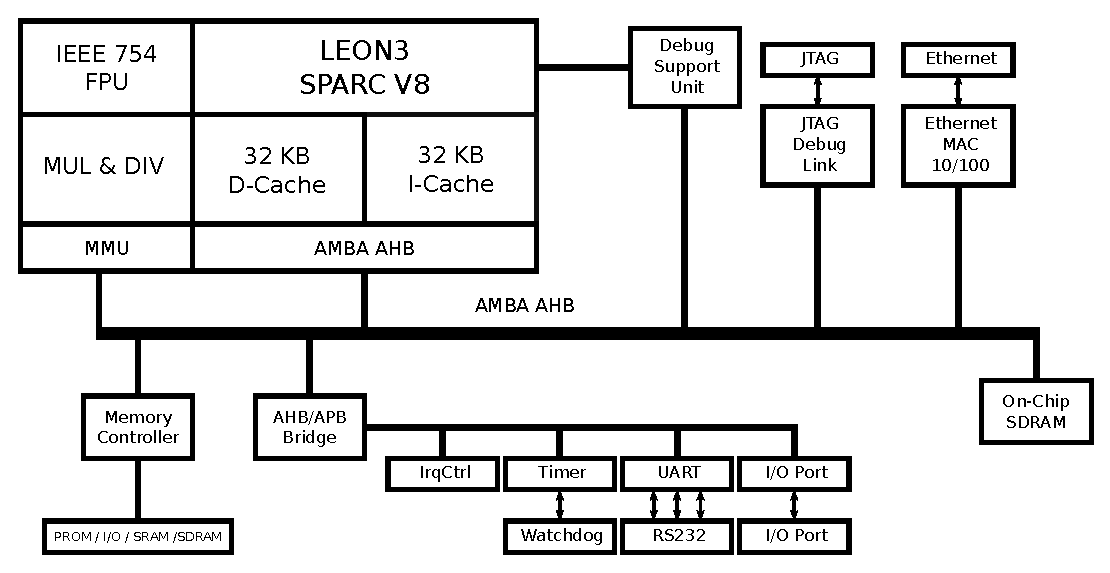
\includegraphics[width=1\textwidth]{Hauptteil/leon3.eps}
\caption{\ac{soc}-Design des LEON3 nach~\cite{comparison}}
\label{fig:leon}
\end{figure}

\subsection{\acl{prhs}}\label{kap:prhs}

Das System der Helmut-Schmidt-Universität, Universität der Bundeswehr Hamburg, ist Befehlssatzkompatibel zu einer \ac{arm}-Architektur. Es bietet die nahezu identischen Bestandteile, wie die
anderen Systeme:\\
\begin{itemize}
  \item \ac{spi} Controller
  \item \ac{uart}
  \item Interrupt-Controller
  \item Instruktionscache
  \item  Timer
  \item Datencache
  \item DDR-Controller
  \item 32-Bit-Prozessorkern
  \item \ac{mmu}
  \item I2C-Controller
  \item Ethernet-Controller
\end{itemize}

Der Prozessor lässt sich durch folgende Eigenschaften näher erläutern:\\
\begin{itemize}
\item \ac{arm}-Architektur typische 16 mal 32-Bit-\emph{General-Purpose}-Register
\item 32-Bit-Befehlswort mit drei Operanden und verschiedenen \ac{arm}-Adressierungsmodi
\item 32-Bit-Adressbus
\item \ac{fpu} in der Entwicklung
\item ein eigenes \ac{prhs}-Bus-System
\item Little-Endian Unterstützung
\item Optionale \ac{mmu}, sowie separate, konfigurierbare Daten- und Instruktionscaches
\item Multicore-fähig
\end{itemize}

\begin{figure}[H]
\centering
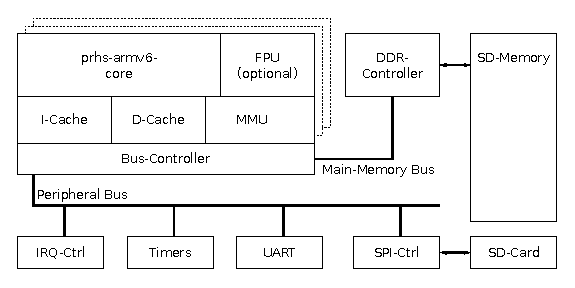
\includegraphics[width=1\textwidth]{Hauptteil/prhs.eps}
\caption{\ac{soc}-Design des \ac{prhs}}
\label{fig:prhs}
\end{figure}


\subsection{lowRISC}\label{kap:lowrisc}
Als viertes System sollte das lowRISC-System die gleichen Benchmarks durchlaufen wie die anderen Systeme. Nachdem die Konfiguration erfolgreich auf das Nexys4-DDR-Board angepasst
und Linux erfolgreich getestet wurde, musste leider im weiteren Verlauf festgestellt werden, dass das System nicht für einen Vergleich dieser Art vorgesehen ist. Es soll langfristig als vollständig
und offenes \ac{soc} dienen und als Low-Cost-Entwicklungsboard zur Verfügung gestellt werden, um die Open-Source-Community zu unterstützten.\\
Hierdurch versprechen sich die Entwickler neue Hardware-Sicherheitsfunktionen erkunden und fördern zu können. Des Weiteren soll es aufstrebenden und soliden Unternehmen die Möglichkeit bieten,
Entwürfe zu erzeugen und diesen Prozess zu vereinfachen. Dazu zählen die Veröffentlichunug von Skripten, Tools, Quellen und Erfahrungen.\\
Ein wesentliches Problem dieses Design auf dem, in dieser Arbeit verwendeten, Board zu benchmarken, war es, dass es Timingprobleme zwischen der System- und der Realzeit gab, sodass Tests,
welche über die Zeit gemessen wurden, nicht korrekt waren. Nachdem versucht wurde diese Probleme durch erneute Rekonfiguration zu lösen und dies auch teilweise gelang, waren die erzielten Ergebnisse
nicht konkurrenzfähig und zeigte erneut, dass dieses System zur Entwicklung genutzt wird und auf Grund dessen, dass es Open-Source ist, noch einige Optimierungsmöglichkeiten bietet.\\

\newpage
\section{Übersicht der getesteten Konfiguration}\label{kap:getestetekonfiguration}


\begin{table}[H]
\centering
\begin{tabular}{|l|c|c|c|c|}
  \hline
  \textbf{Kategorie} & \textbf{Microblaze} & \textbf{LEON3}& \textbf{PRHS}& \textbf{lowRISC}\\
  \hline
  \textbf{Maximale Frequenz} &250 & 183 & 75 & 185\\
  \hline
  \textbf{Pipeline} & 7-Stages & 7-Stages & 5-Stages & 5-Stages\\
  \hline
  \textbf{Architektur} & Microblaze & Sparc V8  & ARM &  Risc\\
  \hline
  \textbf{Sprache} & VHDL & VHDL & VHDL & VHDL\\
    \hline
  \textbf{Address/Daten-Bus} & 32-Bit & 32-Bit & 32-Bit & 64-Bit\\
      \hline
\end{tabular}
  \caption{Eingeschaften der Soft-Core Prozessoren~\cite{comparison}}
 \label{tab:features}
  \end{table}

Des Weiteren wurde bei der Konfiguration darauf geachtet, dass alle Systeme folgende Bestandteile besitzen:\\
\begin{itemize}
  \item \ac{mmu}
  \item 4KB Instruktions- und Datencache
  \item Debug Modul
  \item Interrupt Controller
  \item \ac{spi} Flash Interface
  \item Timer
  \item \ac{uart}-Interface
\end{itemize}

Eine komplett identische Konfiguration aller Systeme war nicht in allen Beobachtungspunkte möglich. So konnte der LEON3 nicht ohne \ac{fpu} konfiguriert werden, da die Benchmarks ohne diese
keine Ergebnisse errechnen konnten. Zum besseren Vergleich wurde dieses System sowohl als Single-, als auch als Dual-Core synthetisiert und getestet. Ein Quad-Core-System war nicht möglich,
da dass Design mehr Ressourcen benötigt, als der \ac{fpga} zur Verfügung stellt. Ebenfalls stellt die Konfiguration
des Caches ein Problem dar, da ein 4 KB-Direct-Mapped-Cache nicht realisierbar ist. Das Konfigurationstool lässt lediglich einen 2-Wege-Assoziativ-Cache zu, welcher die Größe von jeweils 4 KB
zur Verfügung stellt.\\\\
Das \ac{prhs}-System bietet zum jetztigen Zeitpunkt keine \ac{fpu} an, ist jedoch im Vergleich zu den anderen Systemen in der Lage, ein Single-, Dual- und Quad-Core-System zu realisieren,
 welcher erfolgreich geprüft werden konnte.\\
 Der Microblaze ist nicht ohne Weiteres als Multi-Core-System zu konfigurieren, sodass sich alle Benchmarks auf ein Single-Core-System beziehen. Bei diesem System war es jedoch möglich,
 die Tests mit, sowie ohne \ac{fpu} durchzuführen.\\



\section{Synthese-Ergebnisse}\label{kap:synthese}
Wie in Kapitel~\ref{kap:fpga} beschrieben, bietet der \ac{fpga}-Baustein einen begrenzte Anzahl an Ressourcen. So stellt der Flächenverbrauch eine der wichtigen Messgrößen zur Auswahl des
optimalen Systems dar. In diesem Kapitel wird der Flächenverbrauch der verschiedenen Konfigurationen gemessen und dargestellt. Hierbei gibt es je nach System verschiedene Ergebnisse, je nachdem
ob eine \ac{fpu} konfiguriert wurde oder nicht.\\

\textbf{Microblaze}\\
In diesem Abschnitt wird der Ressourcen-Vebrauch des Microblaze-Systems gemessen. Das System wurde, wie bereits beschrieben sowohl mit, als auch ohne \ac{fpu} konfiguriert.
Die Abbildung~\ref{fig:ressourcenmb1} zeigt die Hauptkriterien der Bereichsnutzung. Dabei wurden die \ac{lut}, \ac{lutram} und \ac{ff} des \ac{fpga} betrachet.\\

\begin{figure}[H]
\centering
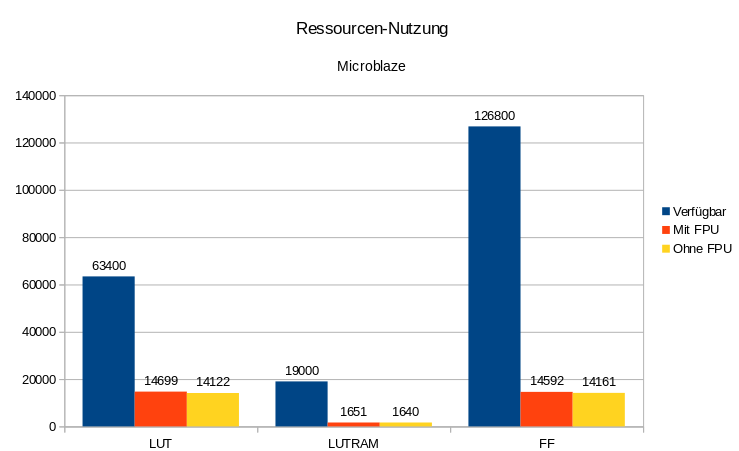
\includegraphics[width=0.6\textwidth]{Hauptteil/ressourcenmb1.png}
\caption{Ressourcen-Nutzung des Microblaze}
\label{fig:ressourcenmb1}
\end{figure}

Wie in~\ref{fig:ressourcenmb1} dargestellt verbrauchen die Konfigurationen 23\%/22\% der \ac{lut}, jeweils 8,6\% der verfügbaren \ac{lutram} und 11,5\%, beziehungsweise 11,2\% der \ac{ff}
innerhalb des \ac{fpga}.\\
Bei diesen Ergebnissen zeigt sich meiner Meinung nach eindeutig, dass es sich um ein kommerzielles System handelt, da der Ressourcen-Verbrauch des Systems mit konfigurierter \ac{fpu}
marginal größer ist. Der Unterschied liegt, bei den Hauptkritieren, bei maximal 1\%(\ac{lut}) erhöhtem Verbrauch an Ressourcen, was darauf schließen lässt, das die \ac{fpu} optimal auf das System
abgestimmt ist.\\

Weitere Ergebnisse sind in~\ref{fig:ressourcenmb2} dargestellt.\\

\begin{figure}[H]
\centering
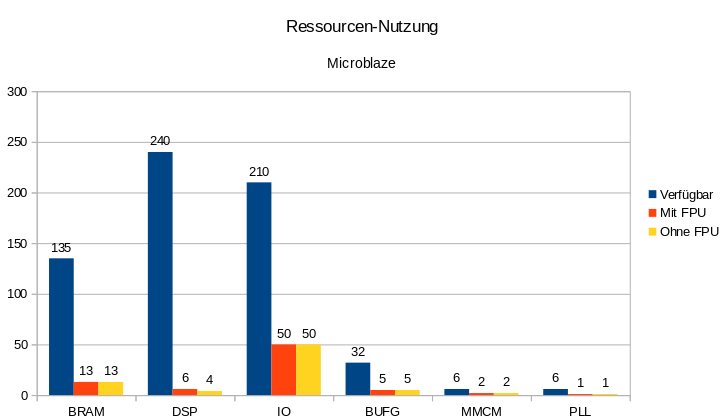
\includegraphics[width=0.7\textwidth]{Hauptteil/ressourcenmb2.png}
\caption{Ressourcen-Nutzung des Microblaze}
\label{fig:ressourcenmb2}
\end{figure}

Daraus resultiert folgende prozentuale Nutzung:\\
\begin{itemize}
  \item \ac{bram}: Jeweils 9,6\%
  \item \ac{dsp}: 2,5\%/1,6\%
  \item \ac{io}-Blöcke: Jeweils 23,8\%
  \item \ac{bufg}: Jeweils 15,6\%
  \item \ac{mmcm} Jeweils 33,3\%
  \item \ac{pll} Jeweils 16,7\%
\end{itemize}

\textbf{LEON3}\\
Auch der Ressourcen-Verbrauch des LEON3 wurde nach der Synthese aufgenommen und in Abbildung~\ref{fig:ressourcenleon31} und~\ref{fig:ressourcenleon32} dargestellt.\\

\begin{figure}[H]
\centering
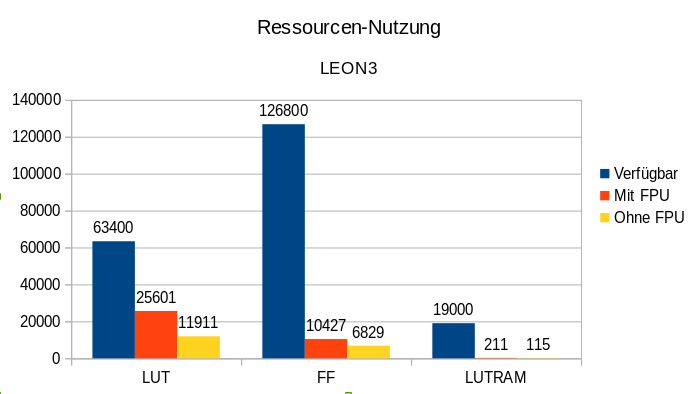
\includegraphics[width=0.7\textwidth]{Hauptteil/ressourcennutzungleon31.png}
\caption{Ressourcen-Nutzung des LEON3}
\label{fig:ressourcenleon31}
\end{figure}

Danach ergibt sich eine Nutzung von 40\%/18,7\% der \ac{lut}, 1,1\%/0,6\% der \ac{lutram} und 8,2\% beziehungsweise 5,4\% der \ac{ff}.
Speziell im Bereich der \ac{lut} und der \ac{ff} ist ein deutlicher Anstieg des Vebrauchs zu beobachten, in dem sich die Zahl der Verbrauchten Ressourcen mehr als verdoppeln (\ac{lut}).
Dieser Unterschied ist dadurch zu erklären, dass es sich um eine IEEE-754-konforme \ac{fpu} handelt, welche die Operanden mmit einfacher und doppelter Genauigkeit unterstüzt. Die Entwickler
beschrieben die \ac{fpu} als ein fortschrittliches Design mit hohem Durchsatz und geringer Latenz und bietet ein umfangreiches Paket an Operationen. Diese Leistungsfähigkeit und der Umfang
führen zu dem starken Unterschied in der Ressourcen-Nutzung.\\

\newpage
Die weiteren Parameter, welche in Abbilduung~\ref{fig:ressourcenleon32} dargestellt sind, unterscheiden sich hingegen nicht voneinander.\\

\begin{figure}[H]
\centering
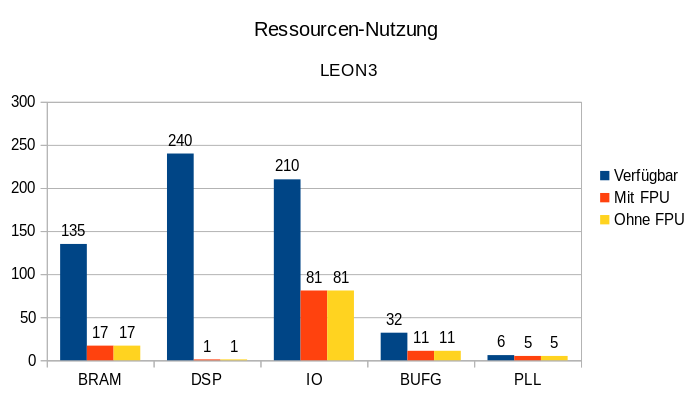
\includegraphics[width=0.7\textwidth]{Hauptteil/ressourcenleon32.png}
\caption{Ressourcen-Nutzung des LEON3}
\label{fig:ressourcenleon32}
\end{figure}

Diese ergeben eine prozentuale Nutzung von:\\
\begin{itemize}
  \item \ac{bram}: Jeweils 12,6\%
  \item \ac{dsp}: Jeweils 0,4\%
  \item \ac{io}-Blöcke: Jeweils 38,6\%
  \item \ac{bufg}: Jeweils 34,4\%
  \item \ac{pll} Jeweils 83,3\%
\end{itemize}

\newpage
\textbf{\acl{prhs}}\\

Da für das \ac{prhs}-System noch keine \ac{fpu} zur Verfügung steht, wurde es ausschließlich ohne \ac{fpu} konfiguriert und getestet.
Um dennoch einen Vergleich zu ermöglichen, wurde das System neben dem Single-Core auch als Dual-Core konfiguriert und getestet.
Die Ergebnisse der Hauptkriterien sind in Abbildung~\ref{fig:ressourcenprhs1} dargestellt.\\

\begin{figure}[H]
\centering
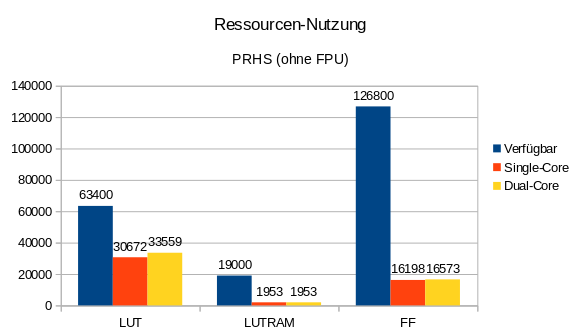
\includegraphics[width=0.7\textwidth]{Hauptteil/ressourcenprhs1.png}
\caption{Ressourcen-Nutzung des \ac{prhs}}
\label{fig:ressourcenprhs1}
\end{figure}

Demnach werden rund 48,4\% der verfügbaren \ac{lut} genutzt. Weiterhin werden 10,3\% des \ac{lutram}, sowie 12,8\% der \ac{ff} für die Konfiguration benötigt. Das Dual-Core-System benötigt
dementsprechend mehr \ac{lut} (52,9\%) und \ac{ff} (13,1\%).
 Auf die in Abbildung~\ref{fig:ressourcenprhs2} dargestellten Parameter hat diese Variation, wie erwartet, keinerlei Einfluss.\\

\begin{figure}[H]
\centering
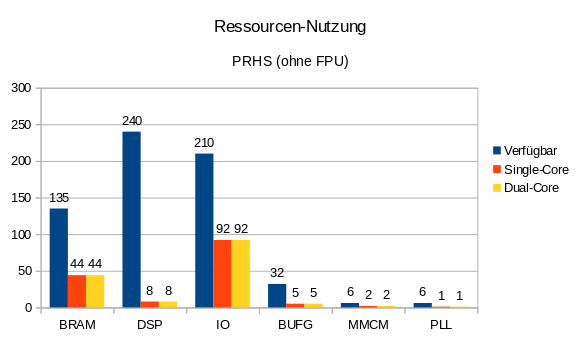
\includegraphics[width=0.57\textwidth]{Hauptteil/ressourcenprhs2.png}
\caption{Ressourcen-Nutzung des \ac{prhs}}
\label{fig:ressourcenprhs2}
\end{figure}

Diese ergeben eine prozentuale Nutzung von:\\
\begin{itemize}
  \item \ac{bram}: 32,6\%
  \item \ac{dsp}:  0,3\%
  \item \ac{io}-Blöcke: 43,8\%
  \item \ac{bufg}: 15,6\%
  \item \ac{mmcm} 33,3\%
  \item \ac{pll} 16,7\%
\end{itemize}


\textbf{Vergleich}

Die Abbildung~\ref{fig:ressourcenresult} stellt den direkten Vergleich der Hauptkritieren grafisch dar.\\

\begin{figure}[H]
\centering
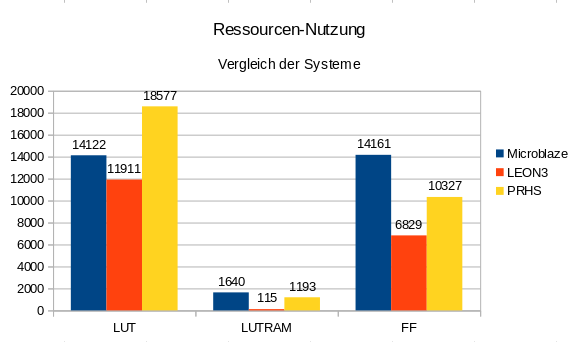
\includegraphics[width=0.7\textwidth]{Hauptteil/ressourcenresult.png}
\caption{Ressourcen-Nutzung der drei Systeme im direkten Vergleich}
\label{fig:ressourcenresult}
\end{figure}

Es ist zu sehen, dass das die kommerziellen Systeme in allen getesteten Bereichen zum Teil deutlich weniger Ressourcen benötigen.
Dies ist damit zu erklären, dass für diese Systeme deutlich mehr finanzielle Mittel bereitstehen und dadurch auch mehr
erfahrenes Personal an der Entwicklung beteiligt sind.\\
Dabei fällt besonders der LEON3 auf, der, zumindest in den Hauptkriterien gegenüber der Konkurrenz, deutlich weniger Ressourcen
benötigt, um die Konfiguration, welche für diesen Vergleich vorgegeben war, zu erfüllen.\\ Jedoch ist im weiteren Verlauf der Tests aufgefallen, dass der LEON3 als Dual-Core deutlich mehr
 der \ac{lut}-Ressourcen (ca. 21.000 Slice \ac{lut} pro Core) benötigt. Das \ac{prhs}-System hingegen benötigt in der Multi-Core-Konfiguration ungefähr 10.000 Slice \ac{lut} mehr pro Core.
Dies führt, wie bereits in Kapitel~\ref{kap:getestetekonfiguration} erwähnt, zu der Schlussfolgerung, dass das LEON3-System auf dem, in dieser Arbeit genutzten, \ac{fpga} nicht realisierbar ist,
auf Grund der begrenzten Ressourcen.\\
 Der Microblaze kommt dem LEON3, bis auf die Anzahl des benötigten \ac{lutram}, sehr nahe und bietet genug Reserven, um das System zu erweitern.\\

\begin{figure}[H]
\centering
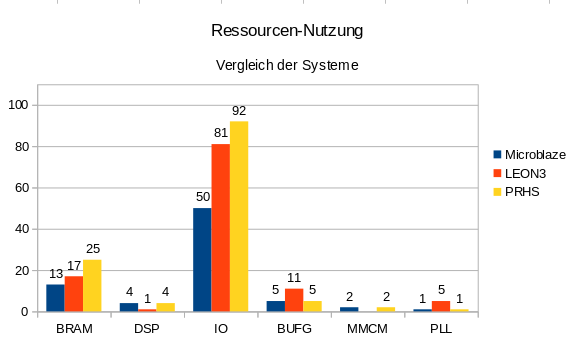
\includegraphics[width=0.7\textwidth]{Hauptteil/ressourcenresult1.png}
\caption{Ressourcen-Nutzung der drei Systeme im direkten Vergleich}
\label{fig:ressourcenresult1}
\end{figure}

Betrachtet man nun in Abbildung~\ref{fig:ressourcenresult1} die restlichen Parameter, bestätigt sich der Eindruck aus der Abbildung
~\ref{fig:ressourcenresult}. Auch hier benötigt das universitätsinterne System mehr Ressourcen als der Microblaze und der LEON3.
Da der LEON3 lediglich mit einem 2-Wege-Assoziativ-Cache konfiguriert werden konnte, erklärt die größere Anzahl an
benötigten \ac{bram}, da in diesem Bereich der Cache realisiert wird.\\
Aufällig ist weiterhin der enorme Verbrauch von \ac{pll}, welcher nach Herstellerangaben zur Generierung der \emph{Main Clock}
benötigt wird.\\

\newpage
\section{Ergebnisse der CoreMark-Benchmark}\label{kap:coremarktest}
Die CoreMark-Benchmark, welche in Kapitel~\ref{kap:coremark} näher beschrieben ist, bietet die Möglichkeit, die Leistung der drei ausgewählten Prozessoren zu messen. Da es, wie beschrieben,
nicht möglich war den LEON3 ohne eine \ac{fpu} zu testen, wurde hier die Anzahl der Prozessoren variiert, sodass die Benchmark sowohl auf einem Single-, als auch auf einem Dual-Core-System
ausgeführt wurde.\\
Das \ac{prhs}-System, welches zur Zeit der Erstellung dieser Arbeit noch nicht über eine funktionieren \ac{fpu} verfügt, wurde ebenfalls als Single- und Dual-Core-System getestet und konnte
darüber hinaus noch als Quad-Core-System getestet werden.\\
Um die Darstellung übersichtlicher zu machen sind die Werte der \emph{Total ticks} an der primären Y-Achsen und die Werte der \emph{Total Time}, beziehungsweise \emph{Iterations/Sec}
an der sekundären Y-Achsen abzulesen.\\

\textbf{Microblaze}\\
Da der Microblaze, wie bereits erwähnt, nicht ohne Weiteres als Multi-Core zu konfigurieren ist, wurde hier das System sowohl mit, als auch ohne \ac{fpu} konfiguriert, um einen
Vergleichswert zu erstellen und um für System an sich darzustellen, inwiefern die \ac{fpu} die Leistung beeinflusst.\\

\begin{figure}[H]
\centering
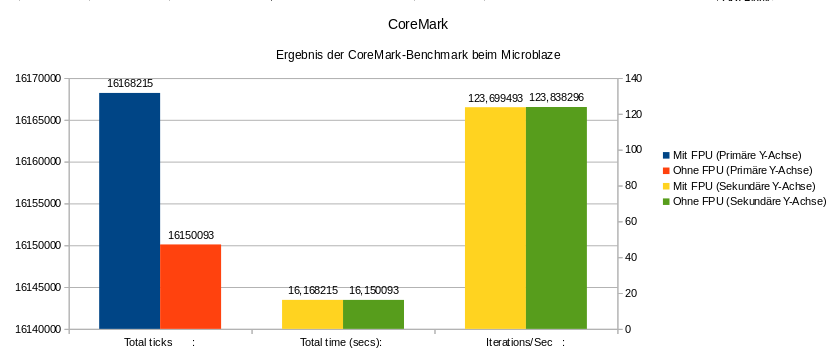
\includegraphics[width=0.7\textwidth]{Hauptteil/coremarkmb.png}
\caption{Ergebnis der CoreMark-Benchmark des Microblaze}
\label{fig:coremarkmb}
\end{figure}


\textbf{LEON3}\\
Die Coremark-Benchmark ist eine Single-Core-Benchmark, dass heißt im Umkehrschluss, dass das Ausführen auf einem Multi-Core-System keinen Einfluss auf das Messergebnis haben sollte.
Um dennoch einen Vergleich zu haben, da ein Test ohne \ac{fpu} nicht möglich war, wurde das System als Single- und Dual-Core konfiguriert und getestet.\\

\begin{figure}[H]
\centering
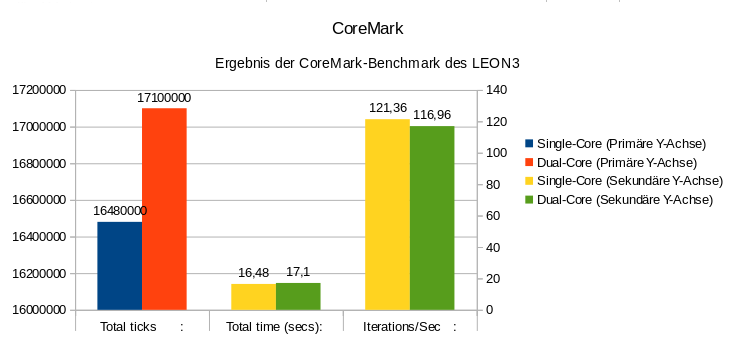
\includegraphics[width=0.7\textwidth]{Hauptteil/coremarkleon3.png}
\caption{Ergebnis der CoreMark-Benchmark des LEON3}
\label{fig:coremarkleon3}
\end{figure}


\textbf{PRHS}\\
Das \ac{prhs}-System bietet zur Zeit der Erstellung dieser Arbeit keine \ac{fpu}, sodass für den Vergleich die hardware neben dem Single-Core, als Dual- und Quad-Core konfiguriert wurde.
Wie bereits beschrieben, hat die Anzahl der Kerne keinen Einfluss auf die Leistungsergebnisse bei dieser Benchmark, jedoch lassen sich Testergebnisse auf diese Art und Weise bestätigen.\\

\begin{figure}[H]
\centering
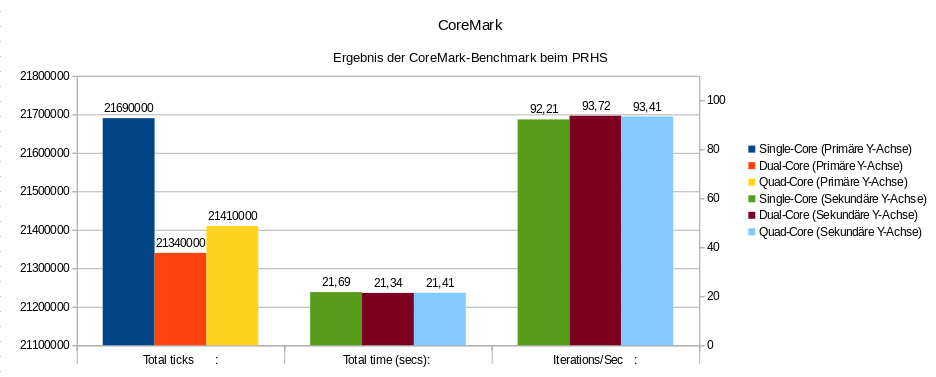
\includegraphics[width=1.1\textwidth]{Hauptteil/coremarkprhs.png}
\caption{Ergebnis der CoreMark-Benchmark des \ac{prhs}}
\label{fig:coremarkprhs}
\end{figure}

\newpage
\textbf{Vergleich}

Die nachfolgende Abbildung~\ref{fig:coremarkresult} stellt nun den direkten Vergleich aller drei Systeme dar.\\

\begin{figure}[H]
\centering
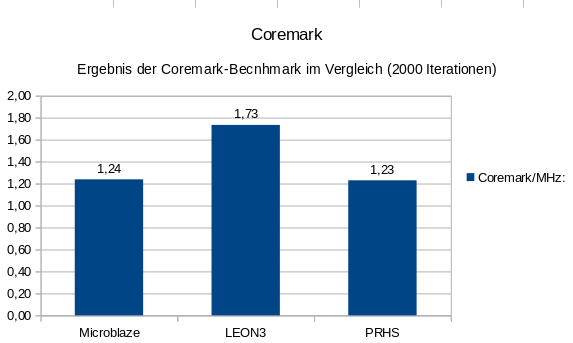
\includegraphics[width=0.7\textwidth]{Hauptteil/coremarkresult.png}
\caption{Coremark-Ergebnis der drei Systeme im direkten Vergleich}
\label{fig:coremarkresult}
\end{figure}

An dieser Grafik lässt sich die Leistungsfähigkeit der \ac{cpu} leicht ablesen, da im Gegensatz zu den einzelnen Diagrammen, das Coremark-Ergebnis durch die jeweilige Taktfrequenz der
einzelnen Systeme dividiert wurde. So ist beispielsweise die Anzahl der Iterationen pro Sekunde beim Prozessor des \ac{prhs} (92,21) geringer als die des Microblaze (123,84), jedoch
relativiert sich die Zahl dadurch, dass der Prozessor des \ac{prhs} mit 75MHz eine geringere Taktfrequenz besitzt, als der Microblaze (100MHz). \\
Der LEON3 erreicht mit einem Wert von 121,36 Iterationen pro Sekunde das zweithöchste Ergebnis, schlägt aber auf Grund der niedrigsten Frequenz (70MHz), die anderen Systeme im direkten Vergleich.\\

\section{Ergebnisse der Dhrystone-Benchmark}\label{kap:dhrystonetest}

Nachdem in Kapitel~\ref{kap:dhrystone} die Funktionsweise der Dhrystone-Benchmark erklärt worden ist, zeigen die Abbildungen~\ref{fig:dhrystonembohnefpu},~\ref{fig:dhrystonesingleleon3} und~\ref{fig:dhrystonesingleprhs} die Ergebnisse
dieser Benchmark. Hierbei wurden in den Grafiken sowohl die \emph{Millisekunden für einen Lauf}, als auch die \emph{\ac{dmips}} dargestellt. Auf der X-Achse der jeweiligen Diagramme ist die Anzahl
der Läufe aufgetragen, welche zwischen 100.000 und 10.000.000 liegen.\\
\newpage

\textbf{Microblaze}

\begin{figure}[H]
\centering
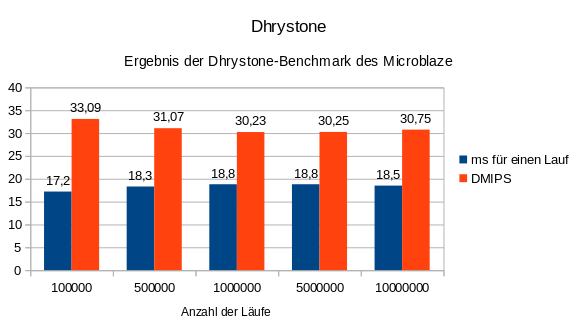
\includegraphics[width=0.7\textwidth]{Hauptteil/dhrystonembohnefpu.png}
\caption{Ergebnis der Dhrystone-Benchmark des Microblaze (ohne \ac{fpu})}
\label{fig:dhrystonembohnefpu}
\end{figure}

In diesem Diagramm ist zu erkennen, dass die Zeiten für einen Lauf, in Millisekunden gemessen, leichte Schwankungen aufweisen, in Abhängigkeit der Anzahl der Läufe. Dies gilt ebenfalls für
die \ac{dmips}-Werte. Der maximale Wert beträgt 33,09 \ac{dmips}, was in etwa 58000 \emph{Dhrystones per second} entspricht.\\

\textbf{LEON3}

\begin{figure}[H]
\centering
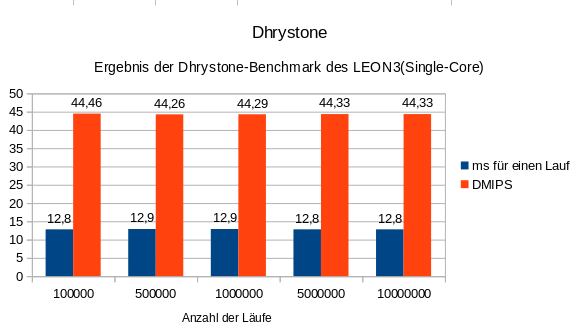
\includegraphics[width=0.7\textwidth]{Hauptteil/dhrystonesingleleon3.png}
\caption{Ergebnis der Dhrystone-Benchmark des LEON3}
\label{fig:dhrystonesingleleon3}
\end{figure}

Der LEON3 erreicht im Vergleich mit 44,46 den höchsten \ac{dmips}-Wert und benötigt am wenigstens Zeit für einen Lauf (12,8-12,9 ms).\\ Die einzelnen Werte der durchgeführten Tests weichen mit
einem Delta von 0,2 \ac{dmips} nur minimal voneinander ab.\\

\textbf{PRHS}

\begin{figure}[H]
\centering
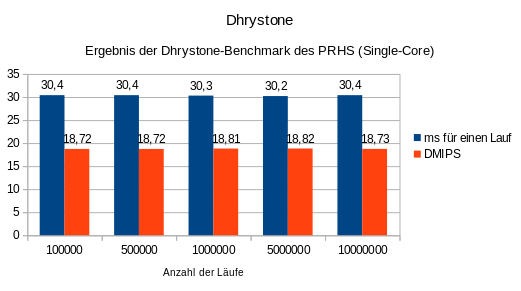
\includegraphics[width=0.7\textwidth]{Hauptteil/dhrystonesingleprhs.png}
\caption{Ergebnis der Dhrystone-Benchmark des \ac{prhs}}
\label{fig:dhrystonesingleprhs}
\end{figure}

Die erreichten Werte des \ac{prhs}-Systems scheinen zwar auf den ersten Blick die niedrigsten zu sein, jedoch relativiert sich die Zahl im abschließenden Vergleich wieder, da die
Coremark-Ergebnisse nur in Verbindung mit der jeweiligen Taktfrequenz der einzelnen Systeme aussagekräftig sind. Das System erreicht einen maximal Wert von
18,82 \ac{dmips} und benötigt für einen Lauf zwischen 30,2 und 30,4 ms.\\

\textbf{Vergleich}


\begin{figure}[H]
\centering
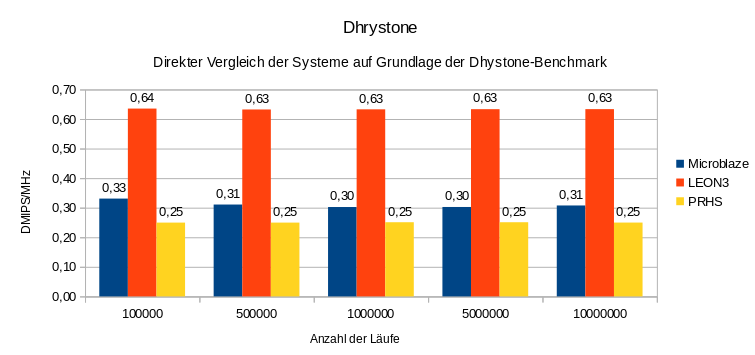
\includegraphics[width=0.7\textwidth]{Hauptteil/dhrystoneresult.png}
\caption{Dhrystone-Ergebnis der drei Systeme im direkten Vergleich}
\label{fig:dhrystoneresult}
\end{figure}

Die Abbildung~\ref{fig:dhrystoneresult} stellt die aussagekräftigsten Werte grafisch dar. Wie bereits erwähnt, gilt für die absoluten \ac{dmips}-Werte zwar je größer, desto besser, jedoch müssen diese
Ergebnisse immer im Verhältnis zu der Taktfrequenz der jeweiligen Systeme gestellt werden. So liegen zwischen den maximalen Werten des Microblaze und des \ac{prhs} 14,27 \ac{dmips}, andererseits
verringert sich der Abstand, wenn man \emph{\ac{dmips}/MHz} betrachtet auf 0,08, da der Microblaze mit 100MHz und das \ac{prhs}-System mit 75MHz getaktet sind.\\
Der LEON3 erzielt konstante Werte, welche mit 0,64 \emph{\ac{dmips}/MHz} zum Teil mehr als doippelt so groß sind, wie die der anderen Systeme. Jedoch gilt es, genauso wie bei dem Microblaze,
zu erwähnen, dass die Ergebnisse, welche auf den Websiten der Hersteller publiziert wurden, nicht ansatzweise erreicht wurden, da diese Systeme die grundlegenden Komponenten enthalten
und ohne Optimierung getestet wurden.\\

\section{Ergebnisse der Ramspeed-Benchmark}\label{kap:ramspeedtest}
Der letzte Benchmark-Test ist der RAMspeed-Test, welcher in Kapitel~\ref{kap:ramspeed} näher beschrieben ist. Diese Grafik zeigt neben der
erreichten Geschwindigkeit, in \emph{MB/s}, auch eindeutig die Größe des Caches, da die Geschwindigkeit signifikant einbringt, wenn die Größe des getesteten Blockes die tatsächliche Größe
des Caches überschreitet. Hierbei ist zu beachten, dass eine Konfiguration des LEON3 mit einem \emph{4 Kb-direct mapped}-Cache nicht möglich war, sodass die Leistung in dem Fall erst nach dem
\emph{8-Kb Block} einbricht.\\

\textbf{Microblaze}

\begin{figure}[H]
\centering
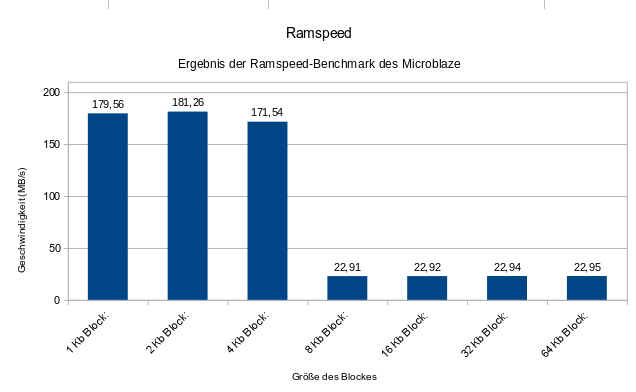
\includegraphics[width=0.65\textwidth]{Hauptteil/ramspeedmicroblaze.png}
\caption{Ergebnis der RAMspeed-Benchmark des Microblaze}
\label{fig:ramspeedmicroblaze}
\end{figure}

Der Microblaze wurde, wie in der gewünschten Konfiguration, mit einem \emph{4-Kb-direct mapped}-Cache synthetisiert. Dies klärt den starken Einbruch in der Geschwindigkeit nach dem 4 Kb-Block.
Die Geschwindigkeit ist nahezu gleichbleibend und erreicht bei einem 2 Kb Block den maxmimalen Wert von 181,26 MB/s.\\

\textbf{LEON3}

\begin{figure}[H]
\centering
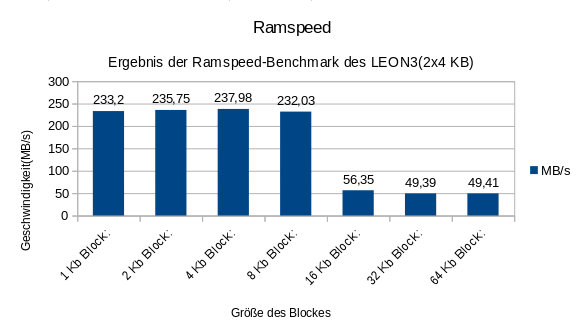
\includegraphics[width=0.7\textwidth]{Hauptteil/ramspeedleon3.png}
\caption{Ergebnis der RAMspeed-Benchmark des LEON3(2\(\times\)4Kb)}
\label{fig:ramspeedleon3}
\end{figure}

Die Ausführung der Ramspeed-Benchmark auf dem LEON3-System ergab eine maximale Geschwindigkeit von 237,98 MB/s. Auch hier ist die Größe des Caches gut anhand des Leistungseinbruches zu erkennen,
wobei dieser auf Grund der insgesamt 8 Kb, erst bei der entsprechenden Größe auftritt.\\

\textbf{PRHS}

\begin{figure}[H]
\centering
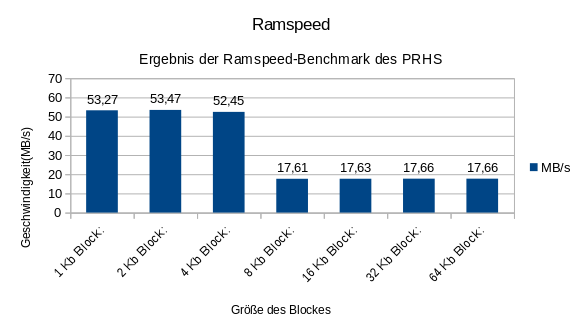
\includegraphics[width=0.6\textwidth]{Hauptteil/ramspeedprhs.png}
\caption{Ergebnis der RAMspeed-Benchmark des \ac{prhs}}
\label{fig:ramspeedprhs}
\end{figure}

Der Cache des \ac{prhs}-Systems wurde, wie der Microblaze, mit einem \emph{4-Kb-direct mapped}-Cache synthetisiert, was durch den Geschwindigkeitseinbruch eindeutig zu sehen ist. Der
Ramspeed-Test ergibt eine maximale Lesegeschwindigkeit von 53,47 MB/s, bei einer Blockgröße von 2 Kb. Die erreichten Ergebnisse befinden sich mit einer Abweichung von maximal 0,98 MB/s
im Toleranzbereich und zeigen eine kontinuierliche Geschwindigkeit an.\\

\textbf{Vergleich}

\begin{figure}[H]
\centering
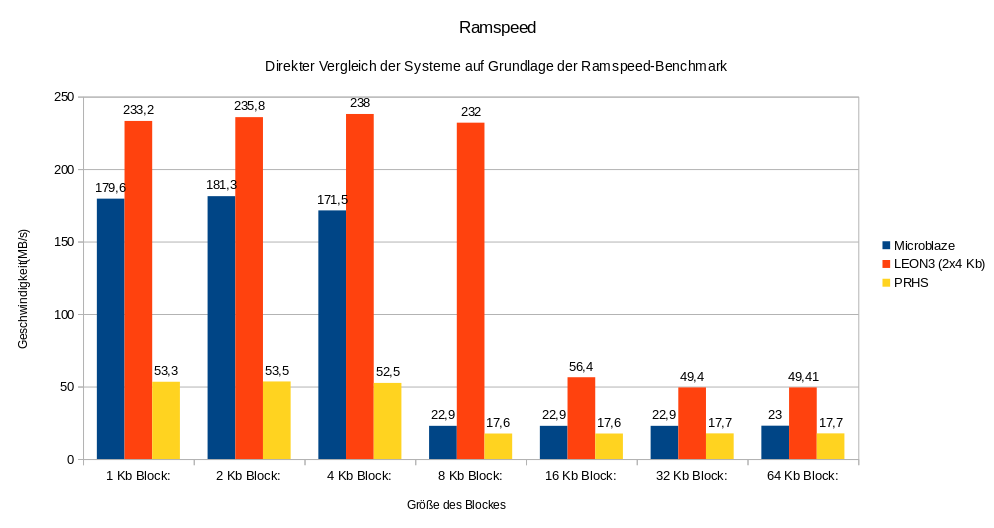
\includegraphics[width=0.7\textwidth]{Hauptteil/ramspeedresult.png}
\caption{Ramspeed-Ergebnis der drei Systeme im direkten Vergleich}
\label{fig:ramspeedresult}
\end{figure}

Die Abbildung~\ref{fig:ramspeedresult} zeigt den direkten Vergleich der drei Systeme bezüglich der erzielten Ramspeed-Benchmark Ergebnisse. Der LEON3 sticht mit seinen erzielten Ergebnissen
heraus, jedoch sind diese gesondert einzuordnen, da dieses System, wie bereits erwähnt, nur als 2-Wege-Assoziativ-Cache, mit einer Gesamtgröße von 8 Kb konfiguriert werden konnte. Nichtsdestotrotz
sind die vom LEON3 erreichten Ergebnisse sehr gut und setzen die Messlatte entsprechend hoch.\\
Der Microblaze, sowie der Cache des \ac{prhs}-Systems sind für den Test identisch konifguriert worden, sodass hier ein direkter Vergleich möglich und aussagekräftig ist.
Der Microblaze erzielt mit 181,3 MB/s, gemessen bei einer Blockgröße von 2 Kb, eine deutlich höhere Geschwindigkeit als der \ac{prhs} (53,5 MB/s) bei gleichbleibender Blockgröße.
Der starke Leistungsunterschied ist auf den ersten Blick überraschend, da alle drei Systeme den gleichen Memorycontroller nutzen. So ist dieser nur durch die Verwendung unterschiedlicher
Bus-Systeme zu erklären. Hierbei nutzt der Microblaze für die Kommunikation zum Cache einen \ac{plb}-Bus, wohingegen das \ac{prhs}-System einen eigenen, für das System entwickelten,
\ac{prhs}-Bus nutzt.

\chapter{Fazit}\label{kap:fazit}

Da die Systeme nicht komplett identisch konfiguriert werden konnten, sind einzelne Benchmark-Tests etwas verzehrt in ihrer Aussagekraft. Beim Vergleich der Ressourcennutzung
anhand der Synthese für das Nexys4-DDR-Board fällt auf, dass das \ac{prhs} am meisten Ressourcen benötigt. Der LEON3 setzt hier Maßstäbe für die Konfiguration als
Single-Core. Dieses Ergebnis relativiert sich jedoch, wenn dieser als Multi-Core konfiguriert wird, da ein Mehrkernsystem so viele Ressourcen benötigt, dass lediglich
ein Dual-Core-System realisierbar ist. An dieser Stelle kann das \ac{prhs} punkten, da eine Mehrkernkonfiguration weniger Ressourcen benötigt als der LEON3 und so
ein System realisiert werden kann, welches bis zu vier Kerne besitzt. Daraus lässt sich schließen, dass das Grundsystem, also das System ohne Prozessor beim \ac{prhs}
deutlich umfangreicher ist als beim LEON3, welcher gleichzeitig einen umfangreicheren Prozessorkern mitbringt. Der Microblaze, welcher als reines Single-Core-System
konfiguriert und bewertet wurde, liegt in der Tabelle der Ressourcennutzung zwischen dem LEON und dem \ac{prhs}. Da dieses System nicht optimiert wurde, sondern
nur alle Optionen konfiguriert wurden, die für diese Arbeit wichtig waren, bietet es sicherlich noch Potenzial zur Verbesserung der Werte.
Des Weiteren ist bei der Konfiguration des LEON3 festzustellen, dass die \ac{fpu} deutlich umfangreicher ist und dadurch mehr Ressourcen benötigt, als die des Microblaze.
Das \ac{prhs} bietet, wie bereits erwähnt, zur Zeit noch keine funktionierende \ac{fpu}. Diese sollte aber, nach aktuellem Entwicklungsstand, bald zur Verfügung stehen.\\
Die Taktfrequenzen der drei Systeme unterscheiden sich allesamt voneiander. So besitzt der LEON3 mit 70 MHz zwar die niedrigste Taktrate, bietet jedoch immer noch genug
Flexibilität die entsprechende Rechenleistung und die Flächenkosten zu vereinen. Das \ac{prhs} taktet sein System mit 75MHz und bietet damit eine stabile Ausführung,
wobei an dieser Stelle sicherlich noch eine Reserve vorhanden ist, die das System schneller taktet. Die höchste Taktfrequenz im Test bietet der Microblaze mit 100 MHz, bei
gleichzeitiger stabiler Ausführung und guten Ergebnissen. Anhand dieses Ergebnisses merkt man den Unterschied zwischen einem Open-Source- und einem kommerziellen System,
da bei dem letztgenannten die einzelnen Komponenten optimal aufeinander abgestimmt sind.\\
Die Abbildung~\ref{fig:coremarkresult} fasst die erreichten Ergebnisse der Coremark-Benchmark grafisch zusammen. In Relation zur jeweiligen Taktfrequenz der Systeme
zeigt sich, dass auch hier der LEON3 mit 1,73 Coremark/MHz den direkten Vergleich für sich entscheiden kann. Mit dem erzielten Wert erreicht der, in dieser Arbeit
konfigurierte LEON3, nahezu das Ergebnis des Herstellers, welcher den LEON3 mit 1,8 Coremark/MHz bewirbt.\cite{leon3} Die Ergebnisse des Microblaze und des \ac{prhs}
sind mit 1,24 Coremark/MHz beziehungsweise 1,23 Coremark/MHz nahezu identisch. Zwar ist der absolute Wert des Microblaze, wie in Abbildung~\ref{fig:coremarkmb} dargestellt,
höher, jedoch relativiert sich dieser, wenn man die Taktfrequenz der jeweiligen Systeme betrachtet. \\
Die Ergebnisse der Coremark-Benchmark, welche größtenteils auf der Dhrystone-Benchmark basiert, werden durch genau diese Benchmark nun bestätigt. Der LEON3 erzielt einen
durchschnittlicher Wert von 0,63 \ac{dmips}/MHz und damit das Beste aller drei Ergebnisse. Den Wert des Herstellers (1,4 \ac{dmips}/MHz) verfehlt er jedoch deutlich,
genau so wie der Microblaze. Dieser erreicht einen Wert von 0,31 \ac{dmips}/MHz bei 100 MHz und somit annähernd halb so viel wie der LEON3. Jedoch gibt Xilinx
auf der Seite des Microblaze~\cite{microblaze} für den Artix-7 einen Wert von 164 \ac{dmips} an, wobei zu diesem Ergebniss keinerlei Erklärung abgegeben werden, bezüglich
Konfiguration und Taktfrequenz. Dies würde bei einer Taktfrequenz von 100 MHz einem Wert von 1,64 \ac{dmips}/MHz entsprechen, welcher sich stark von dem gemessen
Ergebnis unterscheidet. Das \ac{prhs} erreicht einen Wert von 0,25 \ac{dmips}/MHz und bildet damit das schwächste Ergebnis der Benchmark ab, kommt dem Microblaze
bei einer Differenz von 0,06 \ac{dmips}/MHz aber sehr nah.\\
Der letzte Vergleich wurde in der Abbildung~\ref{fig:ramspeedresult} grafisch dargestellt. Hierbei sind lediglich der Microblaze und das \ac{prhs} im direkten Vergleich
zu betrachten, da nur diese beiden System mit einem \emph{4 KB-Direct-Mapped-Cache} konfiguriert wurden, was anhand des Resultats unschwer zu erkennen ist, auf Grund
des Leistungseinbruches nach dem 4 Kb Block. Der Microblaze erreicht einen Spitzenwert von 181,3 MB/s, welcher mehr als dreimal so groß ist, wie der des \ac{prhs}
mit 53,5 MB/s. Dieser Leistungsunterschied ist dadurch zu erklären, dass, wie bereits beschrieben die einzelnen Komponenten des Microblaze optimal aufeinander
abgestimmt sind, dazu zählt vermutlich auch der \ac{plb}-Bus. Das \ac{prhs} hingegen benutzt einen eigenen Bus, des sogenannten \ac{prhs}. Auf Grund dieser Kombination
kann es zu diesem Leistungsunterschied kommen. Der LEON3 fällt, wie bereits erwähnt, auf Grund seines 2-Wege-Assoziativen-Caches aus dem Vergleich raus. Jedoch erzielt
er mit einem Ergebnis von 238 MB/s in der Spitze, einen Wert, welcher besser als der des Microblaze und deutlich besser als der des \ac{prhs} ist.\\ Infolge der
Konfiguration erreicht der LEON3 auf bei einer Blockgröße von 8 Kb nahezu seinen Topwert.\\
Abschließend lässt sich feststellen, dass der LEON3 auf Grund der erreichten Ergebnisse am besten abschneidet, auch wenn das System nicht in allen Punkten
wie gewünscht konfiguriert werden konnte, wie der Cache und die \ac{fpu} gezeigt haben. Nichtsdestotrotz bietet er für eine Open-Source-System eine hohe Stabilität
und erlaubt ein großes Maß an Einstellungsmöglichkeiten und Features. Das Microblaze-System, welches als einziges kommerzielles System getestet wurde, konnte die geforderte
Konfiguration bieten und erreicht gute Ergebnisse im direkten Vergleich. Das System ist in jeglicher Konfiguration sehr stabil und leicht zu konfigurieren, bietet
leider nicht die Möglichkeit ein Multi-Core-System zu realisieren, was für einen direkten Vergleich interessant gewesen wäre. Der \ac{prhs} erreicht dafür, dass er
lediglich an der Helmut-Schmidt-Universtität entwickelt und gefördert wird, sehr gute Ergebnisse und steht dem kommerziellen Microblaze zumindest im Coremark-Vergleich
in nichts nach. Auch was den Umfang des Systems betrifft, kann es sich im direkten Vergleich mit beiden Systemen durchaus messen lassen. Des weiteren war die
Konfigurierbarkeit im Bezug auf Anzahl der Kerne, sowie Größe und Art des Caches einfach zu realisieren.\\
